\documentclass{article}
\usepackage[UTF8]{ctex}
\usepackage{graphicx}
\usepackage{amsmath}
\usepackage{float}
\usepackage{pdfpages} 
\usepackage{hyperref}
\hypersetup{hidelinks,
colorlinks = true,
allcolors = blue,
pdfstartview = Fit,
breaklinks = true}

\usepackage{listings}
\usepackage{color}
\definecolor{dkgreen}{rgb}{0,0.6,0}
\definecolor{gray}{rgb}{0.5,0.5,0.5}
\definecolor{mauve}{rgb}{0.58,0,0.82}
\lstset{frame=tb,
  language=Python,
  aboveskip=3mm,
  belowskip=3mm,
  showstringspaces=false,
  columns=flexible,
  basicstyle={\small\ttfamily},
  numbers=left,%设置行号位置none不显示行号
  %numberstyle=\tiny\courier, %设置行号大小
  numberstyle=\tiny\color{gray},
  keywordstyle=\color{blue},
  commentstyle=\color{dkgreen},
  stringstyle=\color{mauve},
  breaklines=true,
  breakatwhitespace=true,
  escapeinside=``,%逃逸字符(1左面的键),用于显示中文例如在代码中`中文...`
  tabsize=4,
  extendedchars=false %解决代码跨页时,章节标题,页眉等汉字不显示的问题
}


\title{模式识别作业2}
\author{Shi 20159100018}
\date{December 2022}

\begin{document}
\includepdf[pages={1,2,3}]{HandWrite.pdf} 

\maketitle 
本实验所有支撑材料均上传个人GitHub仓库,超链接见脚注\footnote{\href{https://github.com/Shi5013/HomeWork2022/tree/main/PatternRecognition}{code}}

\section{基本内容}
用身高体重数据、或IRIS数据作为本次实验使用的样本集,利用C均值、FCM和层次聚类方法对样本集进行聚类分析,对结果进行分析,从而加深对所学内容的理解和感性认识。
\section{作业要求}
\begin{enumerate}
    \item 同时采用身高和体重数据作为特征,设类别数为2,利用C均值聚类方法对数据进行聚类,并将聚类结果表示在二维平面上。尝试不同初始值对此数据集是否会造成不同的结果。
    \item 对1中的数据利用C均值聚类方法分别进行两类、三类、四类、五类聚类,画出聚类指标与类别数之间的关系曲线,探讨是否可以确定出合理的类别数目。
    \item 对1中的数据利用层次聚类方法进行聚类,分析聚类结果,体会层次聚类方法。
    \item 对1中的数据进行FCM聚类,讨论m对聚类的影响,以及不同聚类个数的合理性。
    \item 对于遗传学数据,分析是否采用父母数据对结果有什么影响。
\end{enumerate}
\section{算法思想及程序实现}
\subsection{算法思想}
\subsubsection{C均值聚类法}
该方法取定C个类别和选取C个初始聚类中心,按最小距离原则将各模式分配到 C类中的某一类,之后不断地计算类心和调整各模式的类别,最终使各模式到其判属类别中心的距离平方之和最小
\subsubsection{层次聚类法}
首先将N个模式视作各自成为一类,然后计算类与类之间的距离,选择距离最小的一对合并成一个新类,计算在新的类别分划下各类之间的距离,再将距离最近的两类合并,直至所有模式聚成两类为止。
\subsubsection{FCM}
根据模糊集合的概念,一个元素隶属于模糊集合不是硬性的,在聚类的问题中,可以把聚类生成的类看成模糊集合,因此,每个样本点隶属于某个类的隶属度就是$[0,1]$区间里面的值。

假定条件及约定,设待分类的模式为$\{\Vec{x}_1,\Vec{x}_2,···\Vec{x}_N,\}$,类的数目$c$事先约定,那么对应的就有$c$个类中心为$V$,每个样本j属于某一类$i$的隶属度为$u_{ij}$
为求约束条件下目标函数的极值,得必要条件如下:
\begin{equation}
    u_{ij} = \frac{1}{\sum\limits_{r=1}^{c}(\frac{d_{ji}}{d_{jr}})^{\frac{2}{m-1}}}
    \label{1}
\end{equation}
\begin{equation}
    v_{i} = \frac{\sum\limits_{j=1}^{n}(u_{ij})^m x_j}{\sum\limits_{j=1}^{n}(u_{ij})^m}
    \label{2}
\end{equation}
用上式循环迭代得到满足要求的聚类中心和隶属度矩阵。
\subsection{算法步骤}
\subsubsection{C均值聚类法}
\begin{enumerate}
    \item[(1)] 任选C个模式特征矢量作为初始聚类中心:\[
    \Vec{z}_1^{(0)},\Vec{z}_2^{(0)},···,\Vec{z}_c^{(0)}, \quad k=0
    \]
    \item[(2)] 将待分类的模式特征矢量集$\Vec{x}_i$中的模式逐个按最小距离原则分划给C类中的某一类,如果$d_{il}^{(k)} = min[d_{ij}^{(k)}] \quad (i = 1,2,...)$,则$\Vec{x}_i\in \omega_l^{(k+1)}$。式中$d_{ij}^{(k)}$表示$\Vec{x}_i$和$\omega_j^{(k)}$的中心$\Vec{z}_j^{(k)}$的距离,上角标表示迭代次数。于是产生新聚类$\omega_j^{(k+1)} (j = 1,2...c)$
    \item[(3)] 计算重新分类后的各类心\[
    \Vec{z}_j^{(k+1)} = \frac{1}{n_j^{k+1}\sum\Vec{x}_i} \quad (j = 1,2...c)
    \]
    式中$n_j^{k+1}$为类$\omega_j^{(k+1)}$中所含模式的个数。
    \item[(4)] 如果$\Vec{z}_j^{(k+1)} = \Vec{z}_j^{(k)},j = 1,2,...,c$,则结束,否则$k = k+1$,转至(2)
\end{enumerate}
\subsubsection{层次聚类法}
\begin{enumerate}
    \item[(1)] 初始分类。令k=0, 每个模式自成一类,即$G_i^{(0)} = \{ \Vec{x}_i \}(i = 1,2,···,N)$
    \item[(2)] 计算各类间的距离$D_{ij}$,由此生成一个兑成距离矩阵$D^{(k)} = (D_{ij})_{m \times m}$,$m$为类的个数(初始时$m=N$)
    \item[(3)] 找出前一步求得的矩阵$D^{(k)}$中最小的元素,设它是$G_i^{(k)}$与$G_j^{(k)}$间的距离,将$G_i^{(k)}$与$G_j^{(k)}$两类合并称一类,于是产生新的聚类$G_1^{(k+1)}$,\\$G_2^{(k+1)} ···$,令$k = k+1,m = m-1$
    \item[(4)] 检查类的个数。如果类数m大于2,转至(2);否则停止。
\end{enumerate}
\subsubsection{FCM}
\begin{enumerate}
    \item[(1)] 设定聚类数目$c$和参数$m$(模糊因子)
    \item[(2)] 给出初始隶属度矩阵$U^{(0)}$($U^{(0)}$各行元素之和应为1,在实验程序给$U^{(0)}$每一列随机赋予$c-1$个0, 1个1)
    \item[(3)]利用式(\ref{2})计算新的聚类中心$V_i$
    \item[(4)]利用式(\ref{1})计算新的隶属度矩阵(若分母存在中$d_{ji} = 0$,则$u_{ij} = 1$,且对$j \neq i,u_{ij} = 0$)
    \item[(5)]用一个矩阵范数比较两次迭代之间隶属度矩阵,如果
    \[
    ||U^{k+1}-U^{k}|| \leq e
    \]则停止迭代,否则转(3)。
\end{enumerate}
\subsection{数据说明}
根据实验材料所给,word文档的表中共52位同学的身高体重数据。即本次聚类分析实验样本数量为52。将实验样本绘制成二维图如下:
\begin{figure}[H]
    \centering
    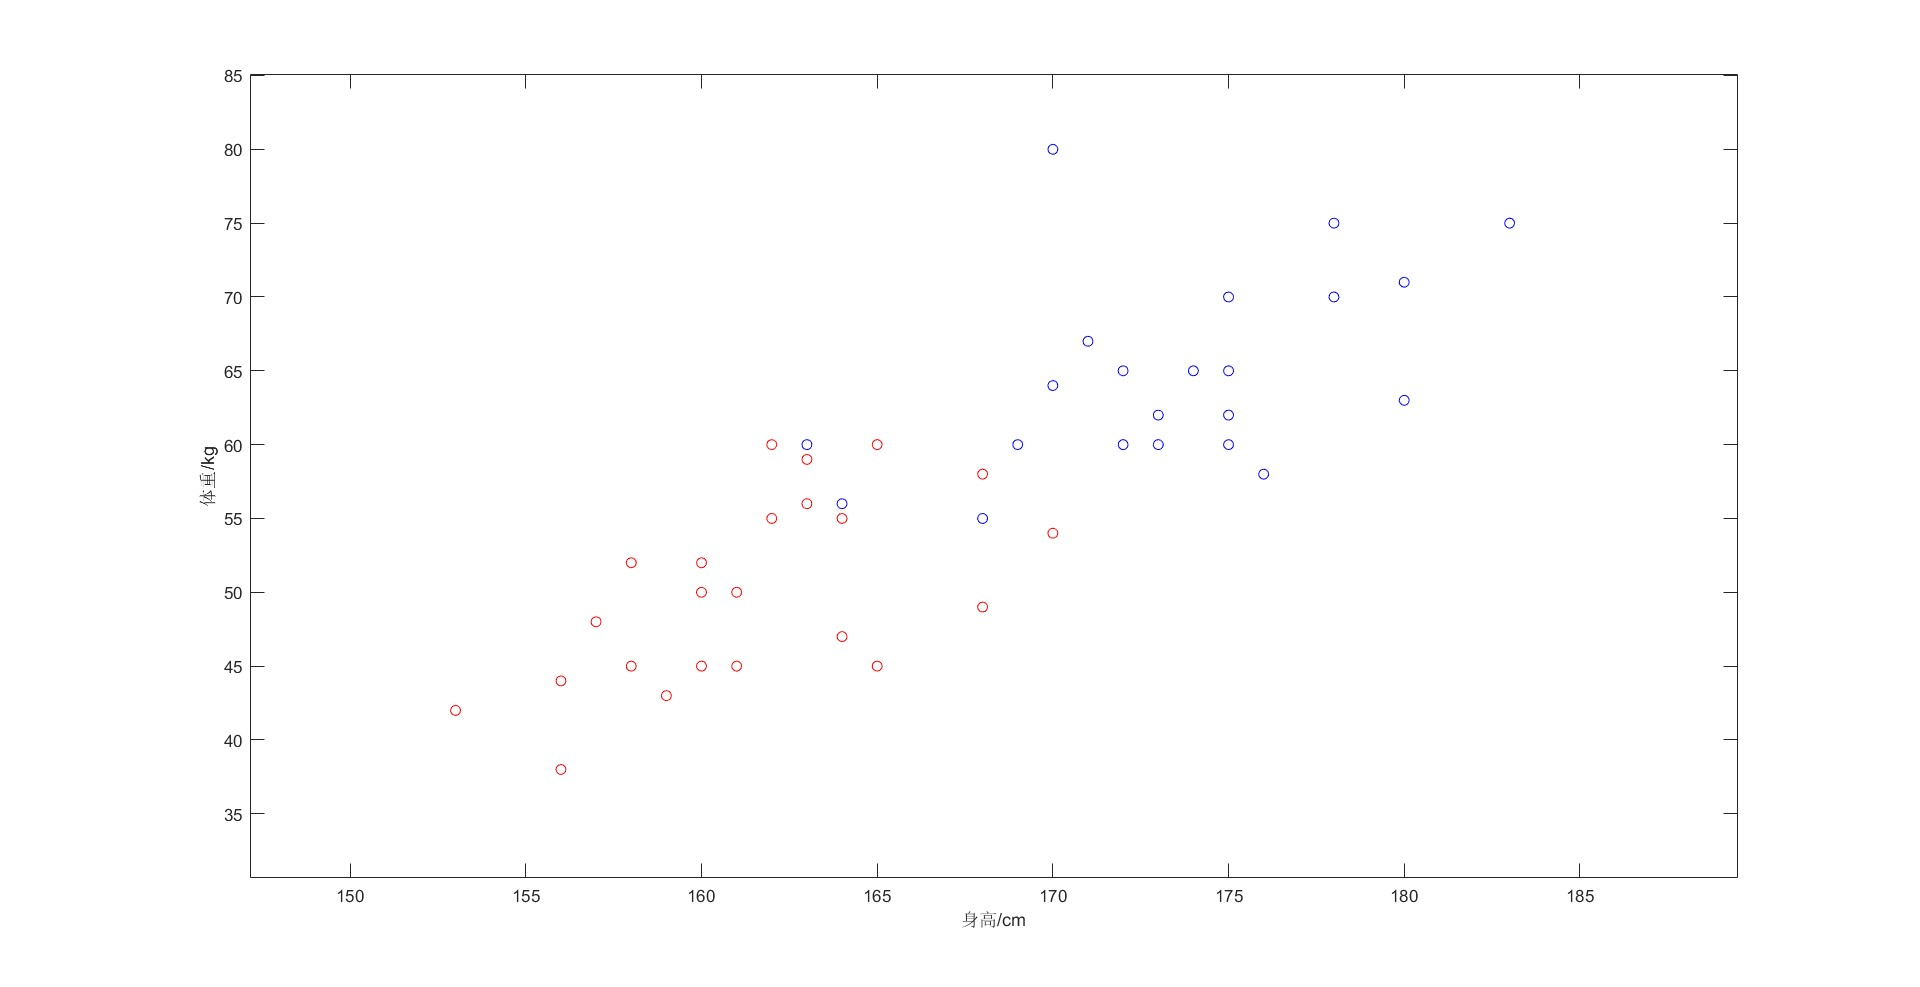
\includegraphics[width=1\textwidth]{image/Figure01.jpg}
    \caption{实验数据,红色为女生,蓝色为男生,各26个}
    \label{Figure01.}
\end{figure}

\subsection{程序实现}
程序实现主要依赖MATLAB中所提供的函数,其中C-means聚类主要使用\verb|kmeans|函数;层次聚类法主要使用\verb|pdist|、\verb|linkage|、\verb|dendrogram|、\verb|cluster|;
FCM主要使用\verb|fcm|。
具体的完整代码与注释见附录,.m文件见GitHub仓库:\quad \href{https://github.com/Shi5013/HomeWork2022/tree/main/PatternRecognition}{code}

\section{实验结果分析}

\subsection{要求1}
利用C-means对数据进行聚类,选择类别数为2。第一次选择第一个男生和第一个女生的身高体重数据,初始聚类中心为:(163,60)(153,42)。得到聚类结果如下。聚类中心为(160.773,48.5455)(172,63.4),\\$J_e = 2.1565e+03$。

\begin{figure}[H]
    \centering
    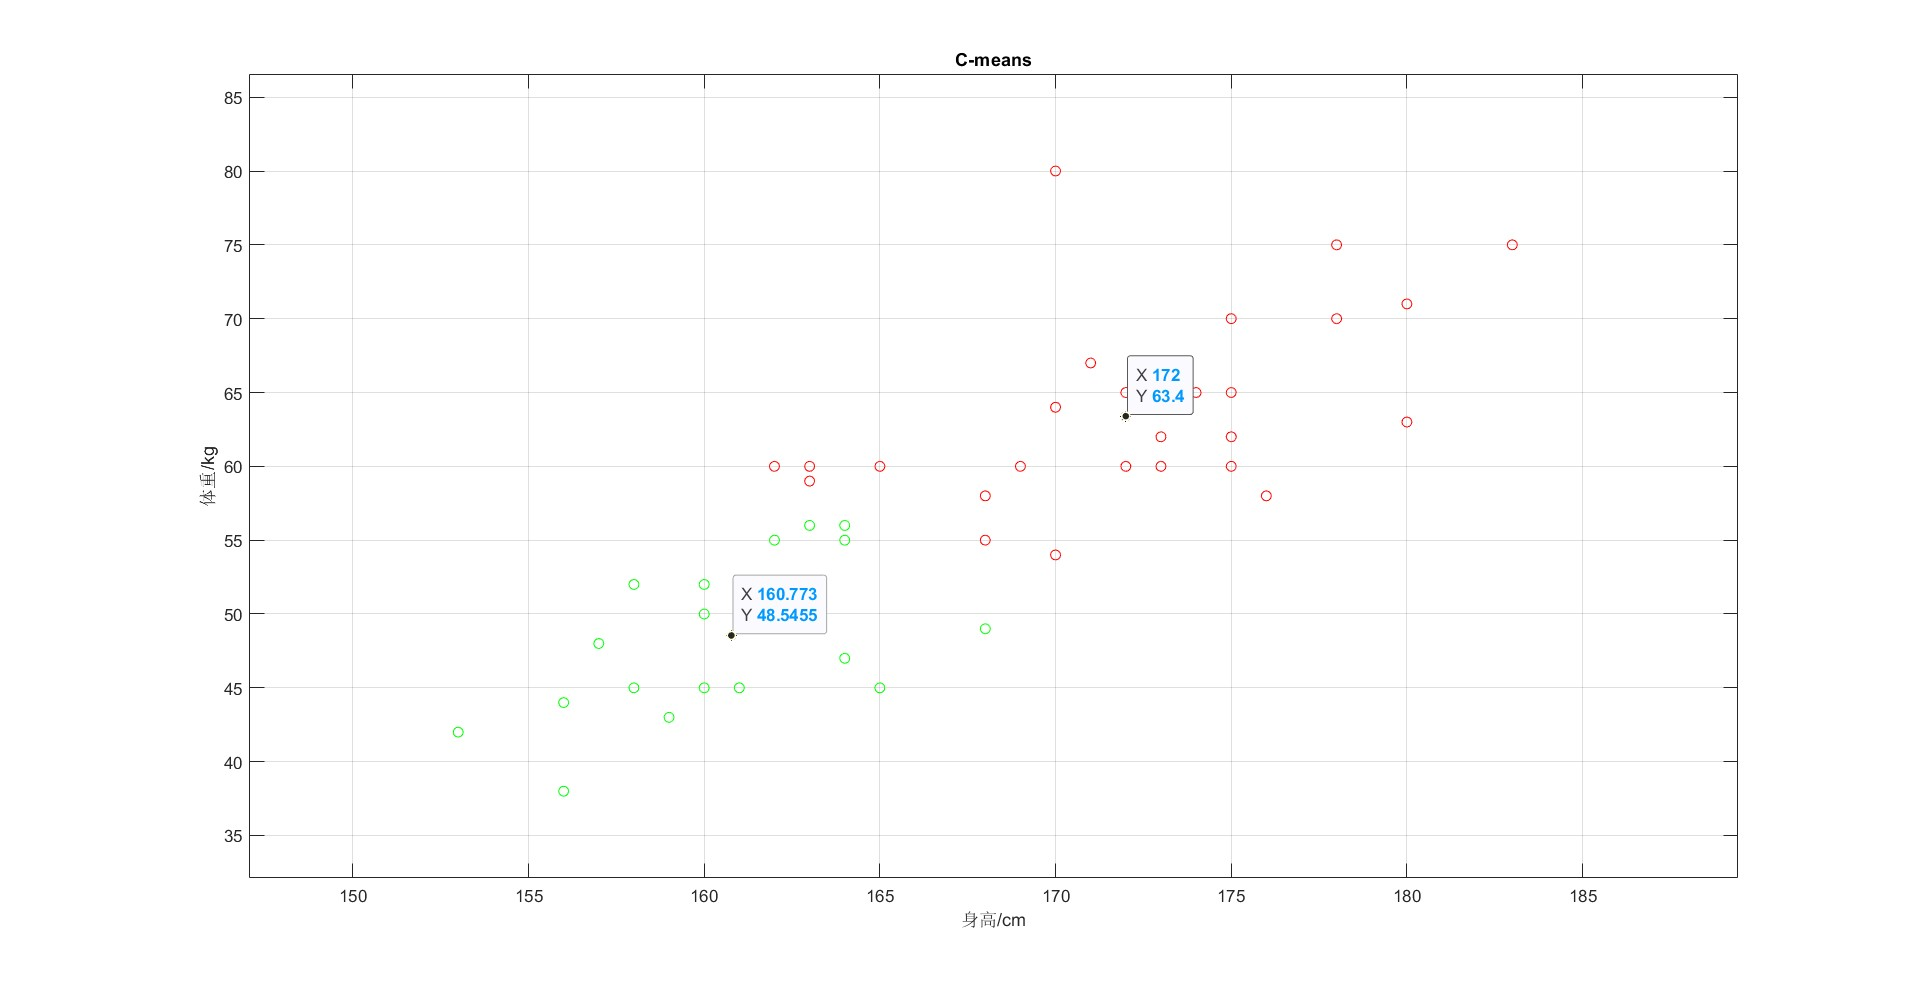
\includegraphics[width=1\textwidth]{image/Figure02.jpg}
    \caption{C=2的第一次聚类结果}
    \label{Figure02}
\end{figure}

第二次选择最后一个男生和最后一个女生,初始聚类中心为:(183,75)(170,54)。得到聚类结果如下。聚类中心为(162.29,51.2258)(174.571,65.8095),\\$J_e = 1.9466e+03$。

\begin{figure}[H]
    \centering
    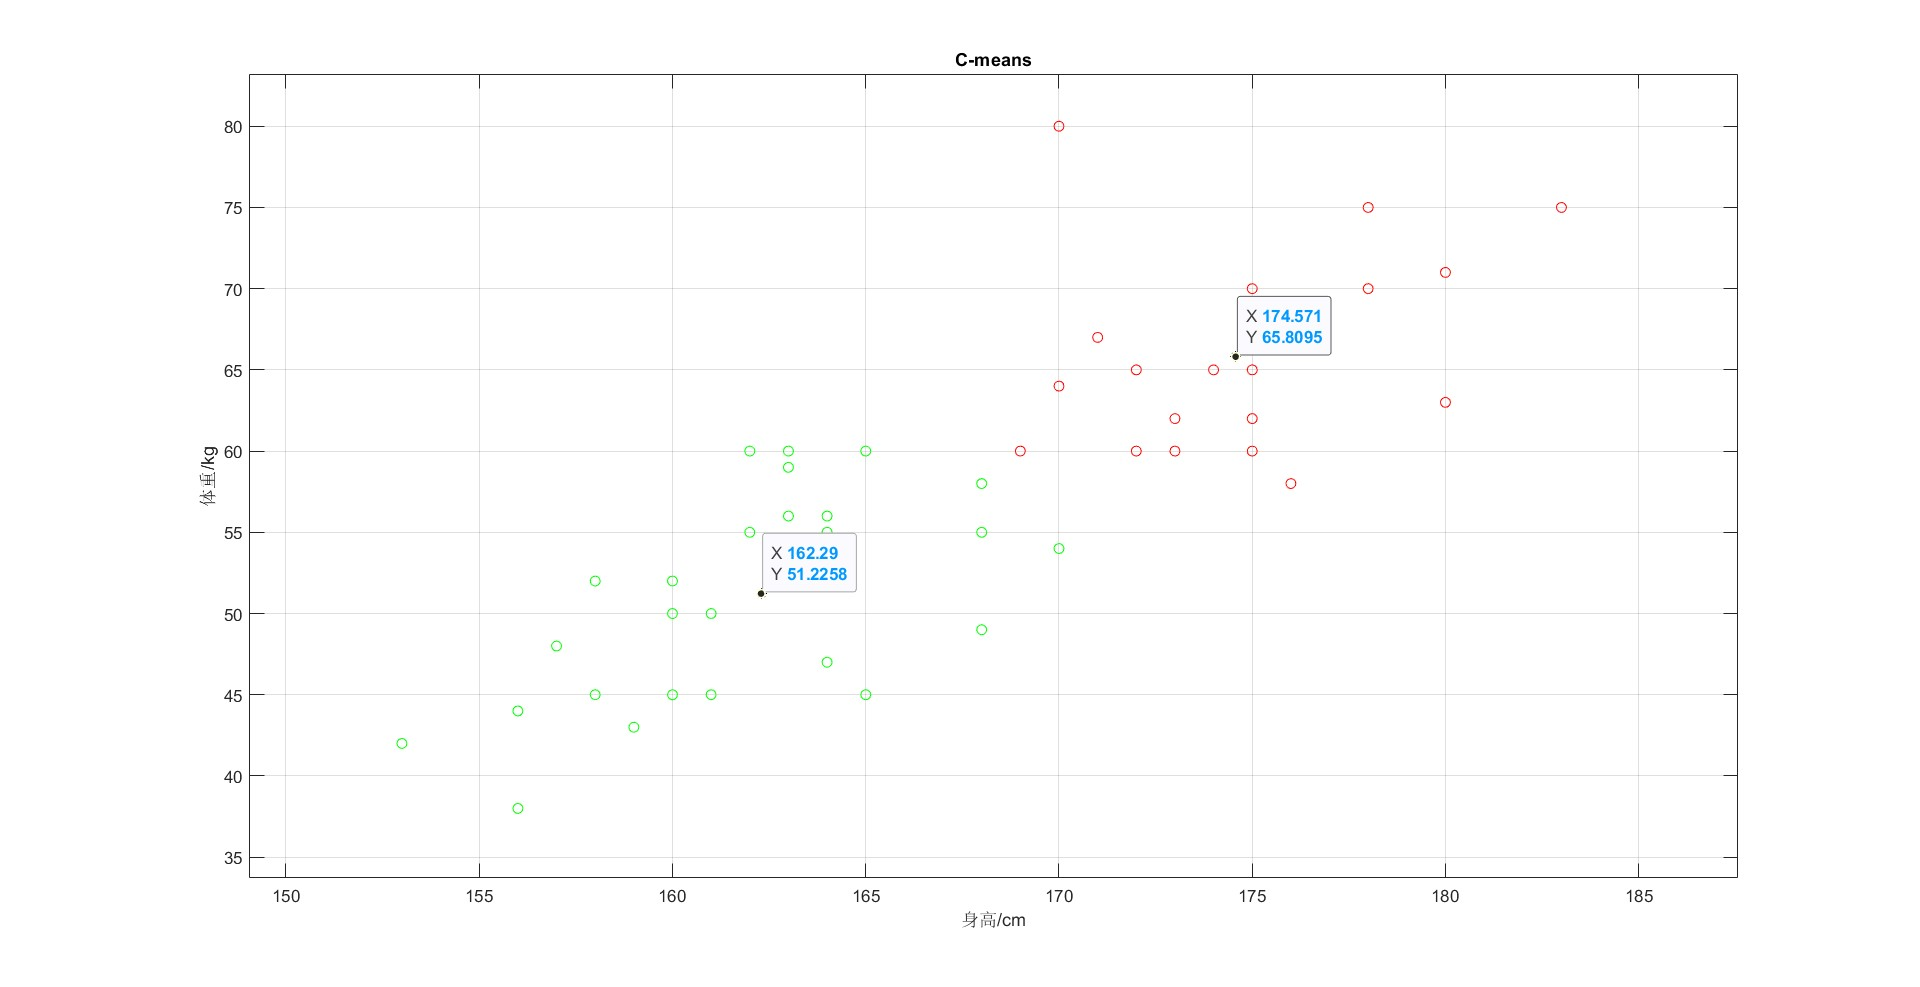
\includegraphics[width=1\textwidth]{image/Figure03.jpg}
    \caption{C=2的第二次聚类结果}
    \label{Figure03}
\end{figure}

第三次选择最后一个男生和第一个女生,初始聚类中心为:(183,75)(153,42).得到聚类结果如下。聚类中心为(162.29,51.2258)(174.571,65.8095),\\$J_e = 1.9466e+03$。

\begin{figure}[H]
    \centering
    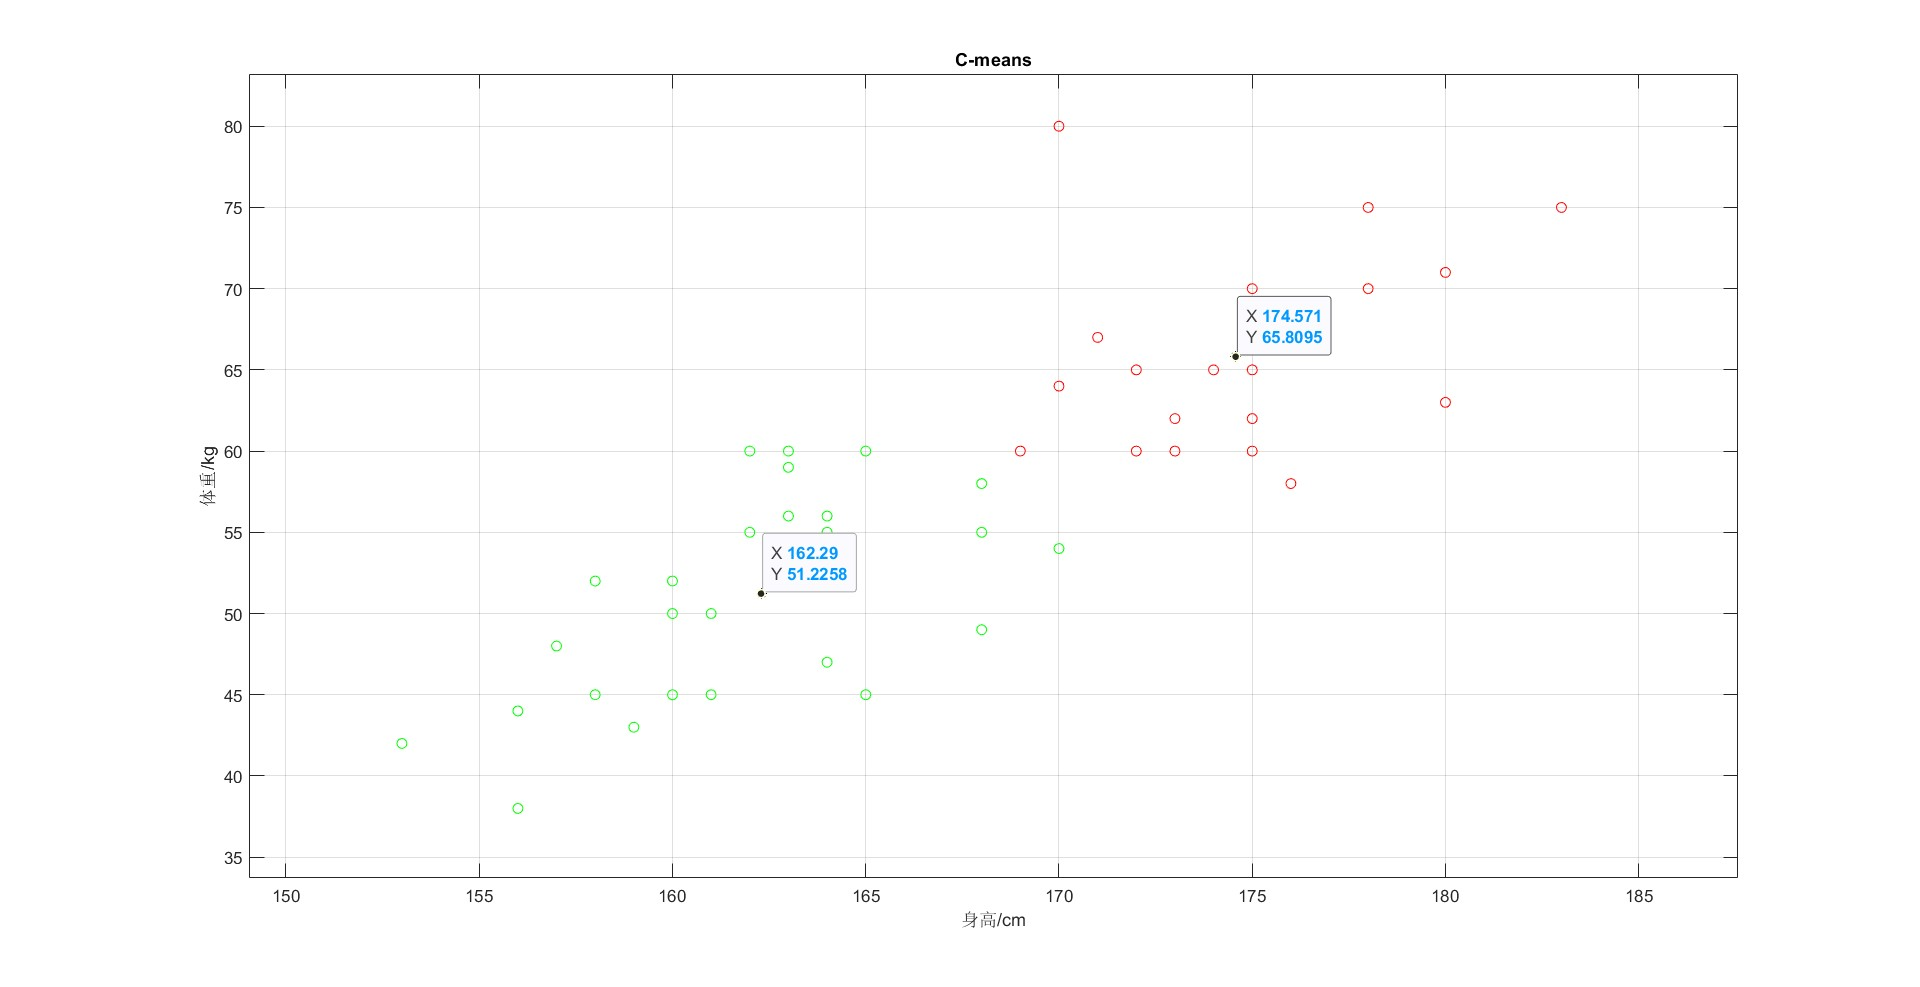
\includegraphics[width=1\textwidth]{image/Figure04.jpg}
    \caption{C=2的第三次聚类结果}
    \label{Figure04}
\end{figure}

通过选择不同的初始聚类中心,可以得到不同的结果,但不同的聚类中心也有可能得到相同的聚类结果。
\subsection{要求2}
选择类别数为3,初始聚类中心为(183,75)(170,54)(153,42)。得到聚类结果如下。聚类中心为:(160.059,46.4706)(167.727,58.2727)(175.846,69.0769).\\$J_e = 903.2275$

\begin{figure}[H]
    \centering
    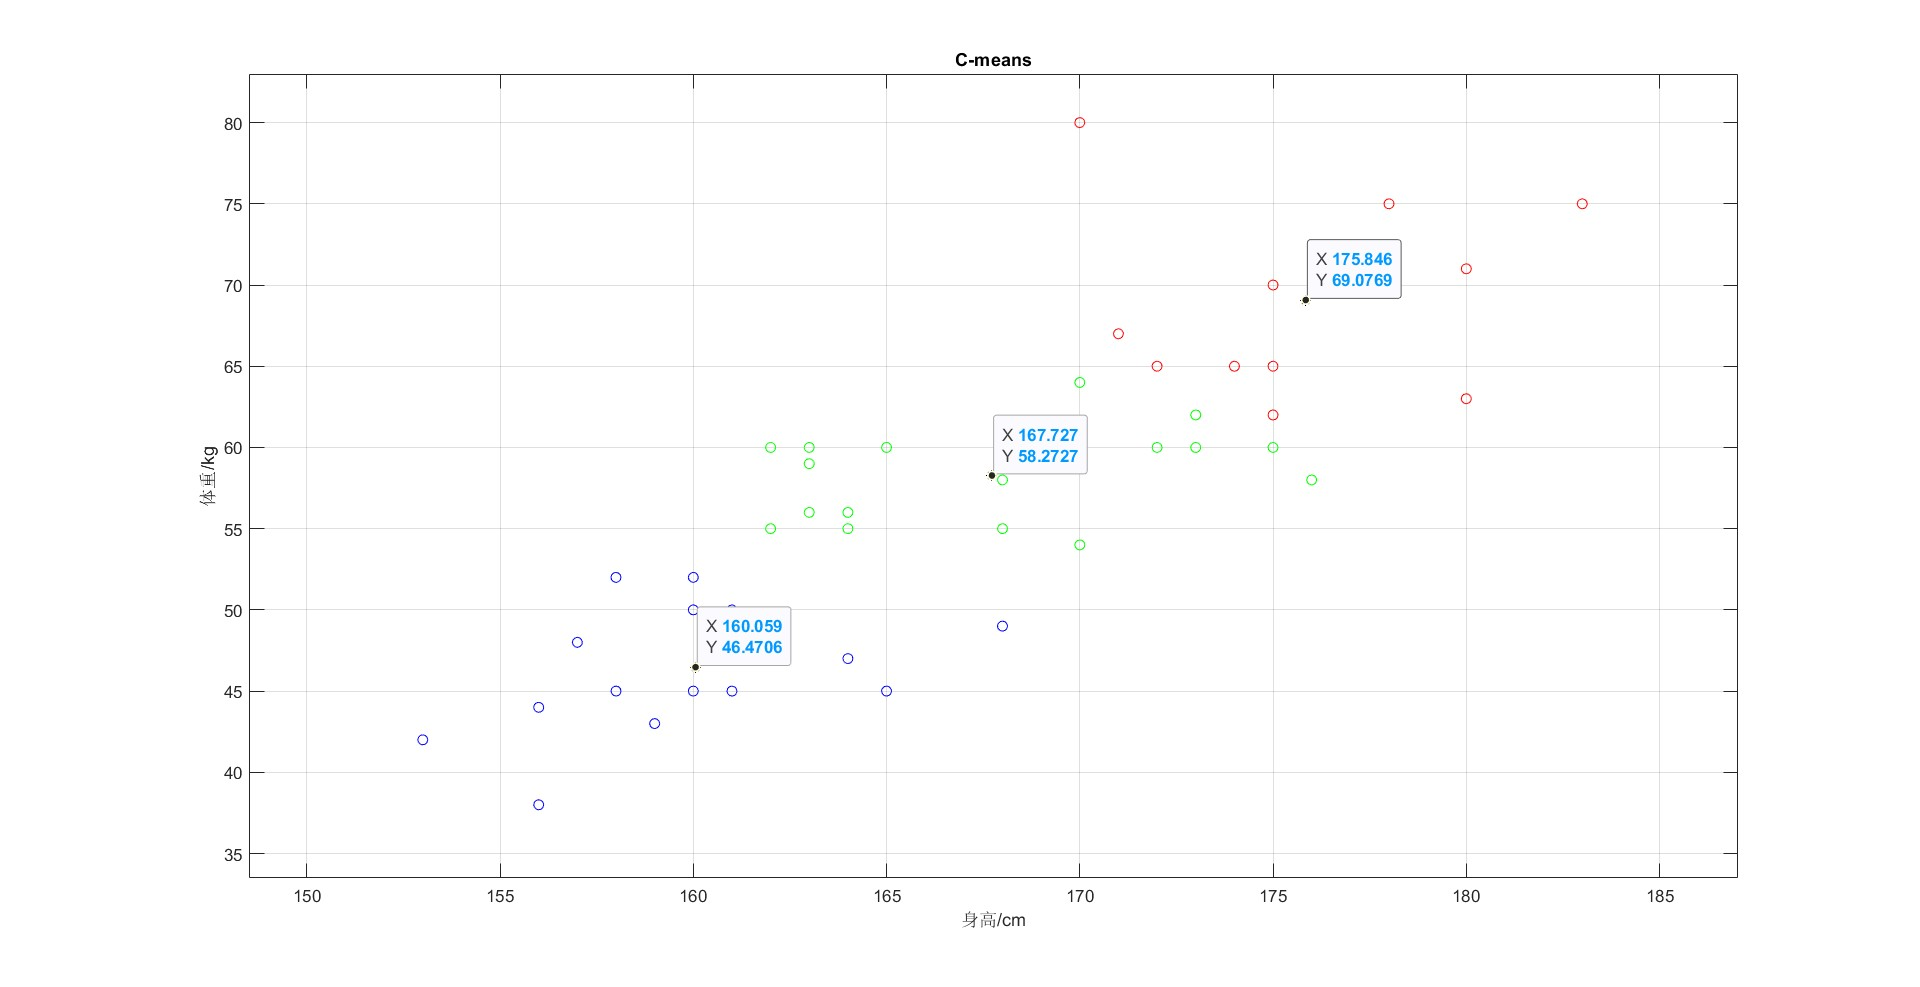
\includegraphics[width=1\textwidth]{image/Figure05.jpg}
    \caption{C=3的聚类结果}
    \label{Figure05}
\end{figure}

选择类别数为4,初始聚类中心为(183,75)(170,54)(163,60)(153,42)。得到聚类结果如下。聚类中心为:(160.059,46.4706)(167.727,58.2727)\\(175.846,69.0769).$J_e = 562.9040$

\begin{figure}[H]
    \centering
    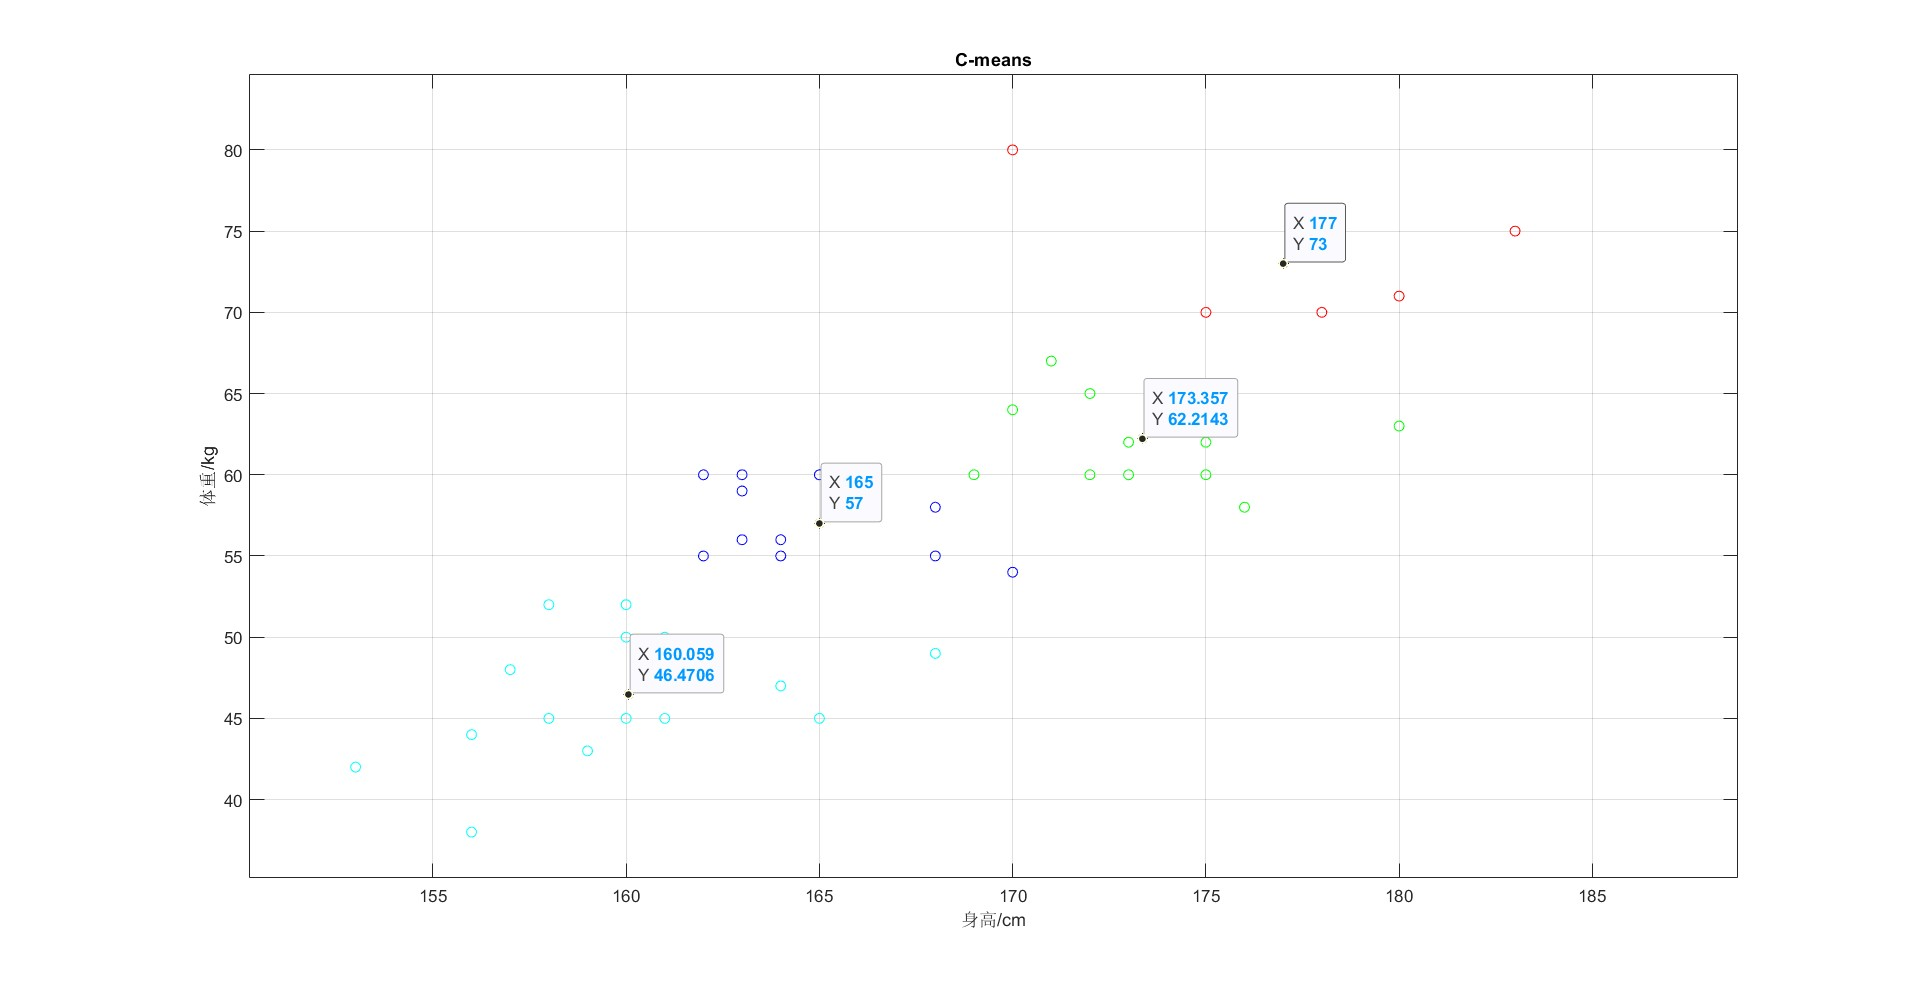
\includegraphics[width=1\textwidth]{image/Figure06.jpg}
    \caption{C=4的聚类结果}
    \label{Figure06}
\end{figure}

选择类别数为5,初始聚类中心为(183,75)(170,54)(163,60)(153,42)(172,60)。得到聚类结果如下。聚类中心为:(160.059,46.4706)(167.727,58.2727)(175.846,69.0769).\\$J_e = 370.8981$

\begin{figure}[H]
    \centering
    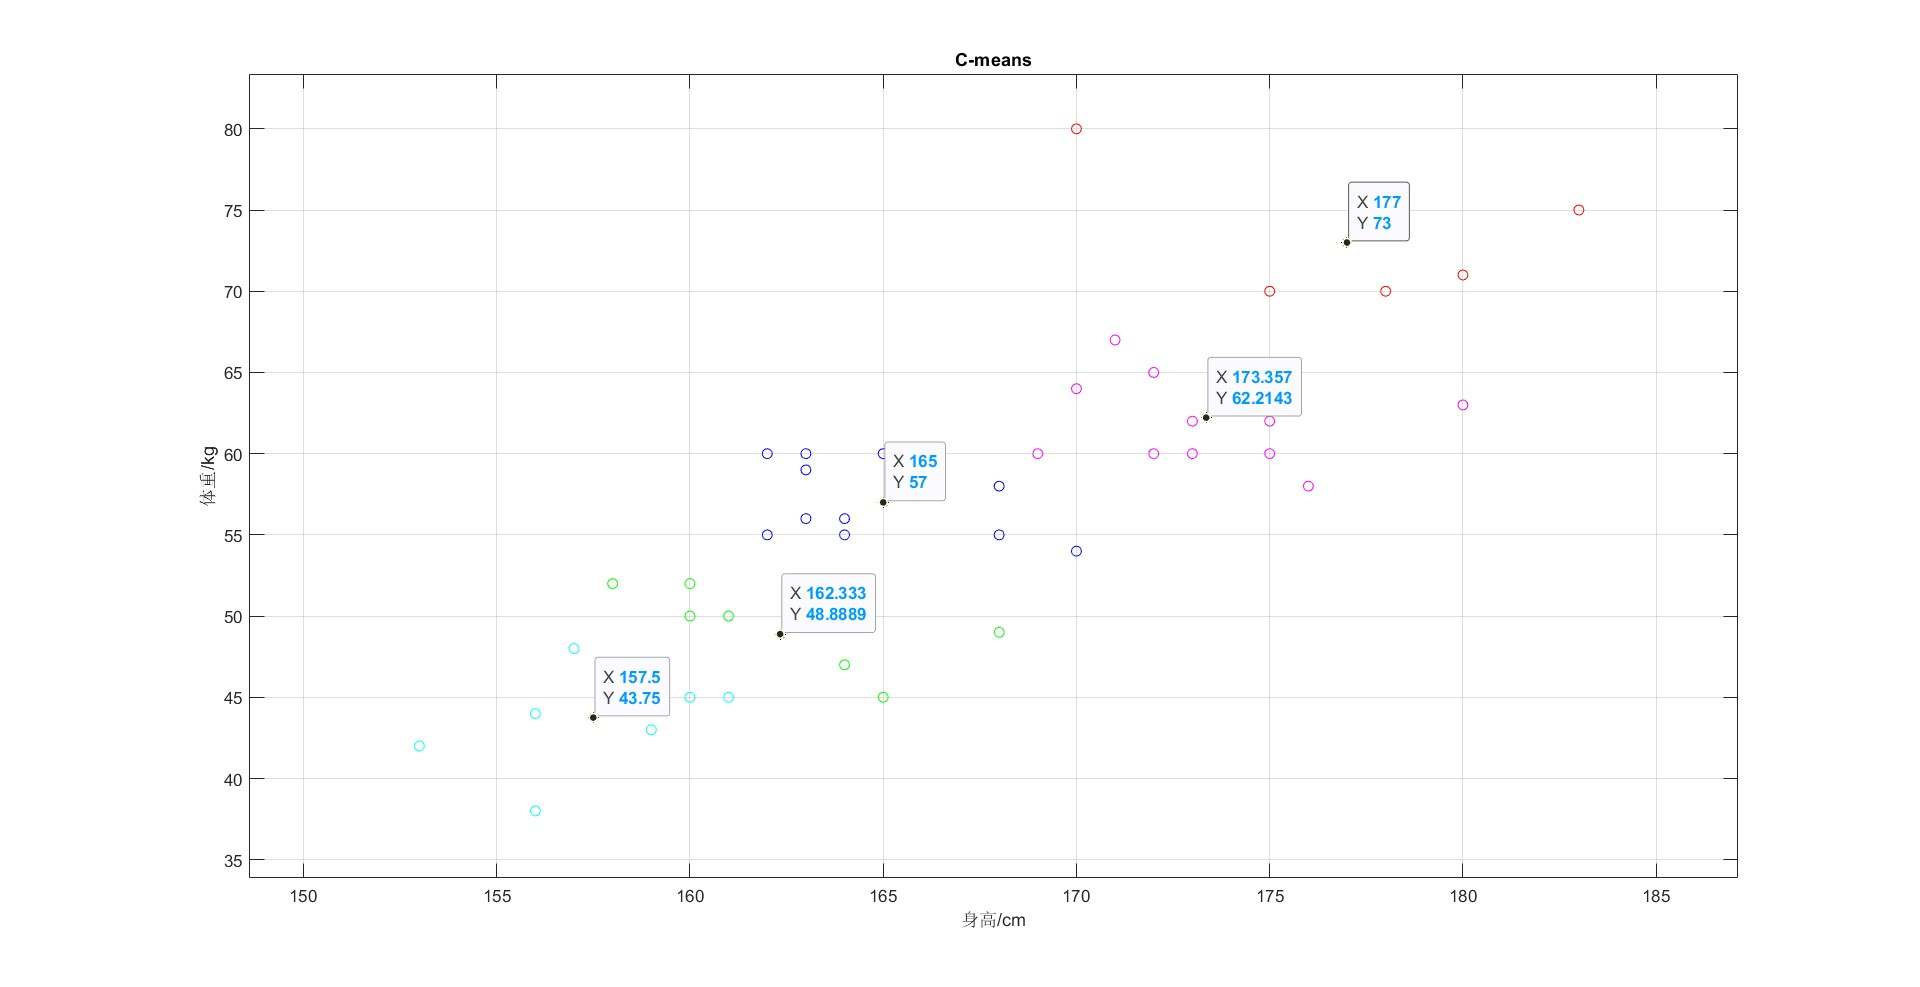
\includegraphics[width=1\textwidth]{image/Figure07.jpg}
    \caption{C=5的聚类结果}
    \label{Figure07}
\end{figure}

画出不同聚类类别数C与$J_e$的函数曲线如下,可以看出,拐点离2较近,所以此样本集聚为二类最佳。

\begin{figure}[H]
    \centering
    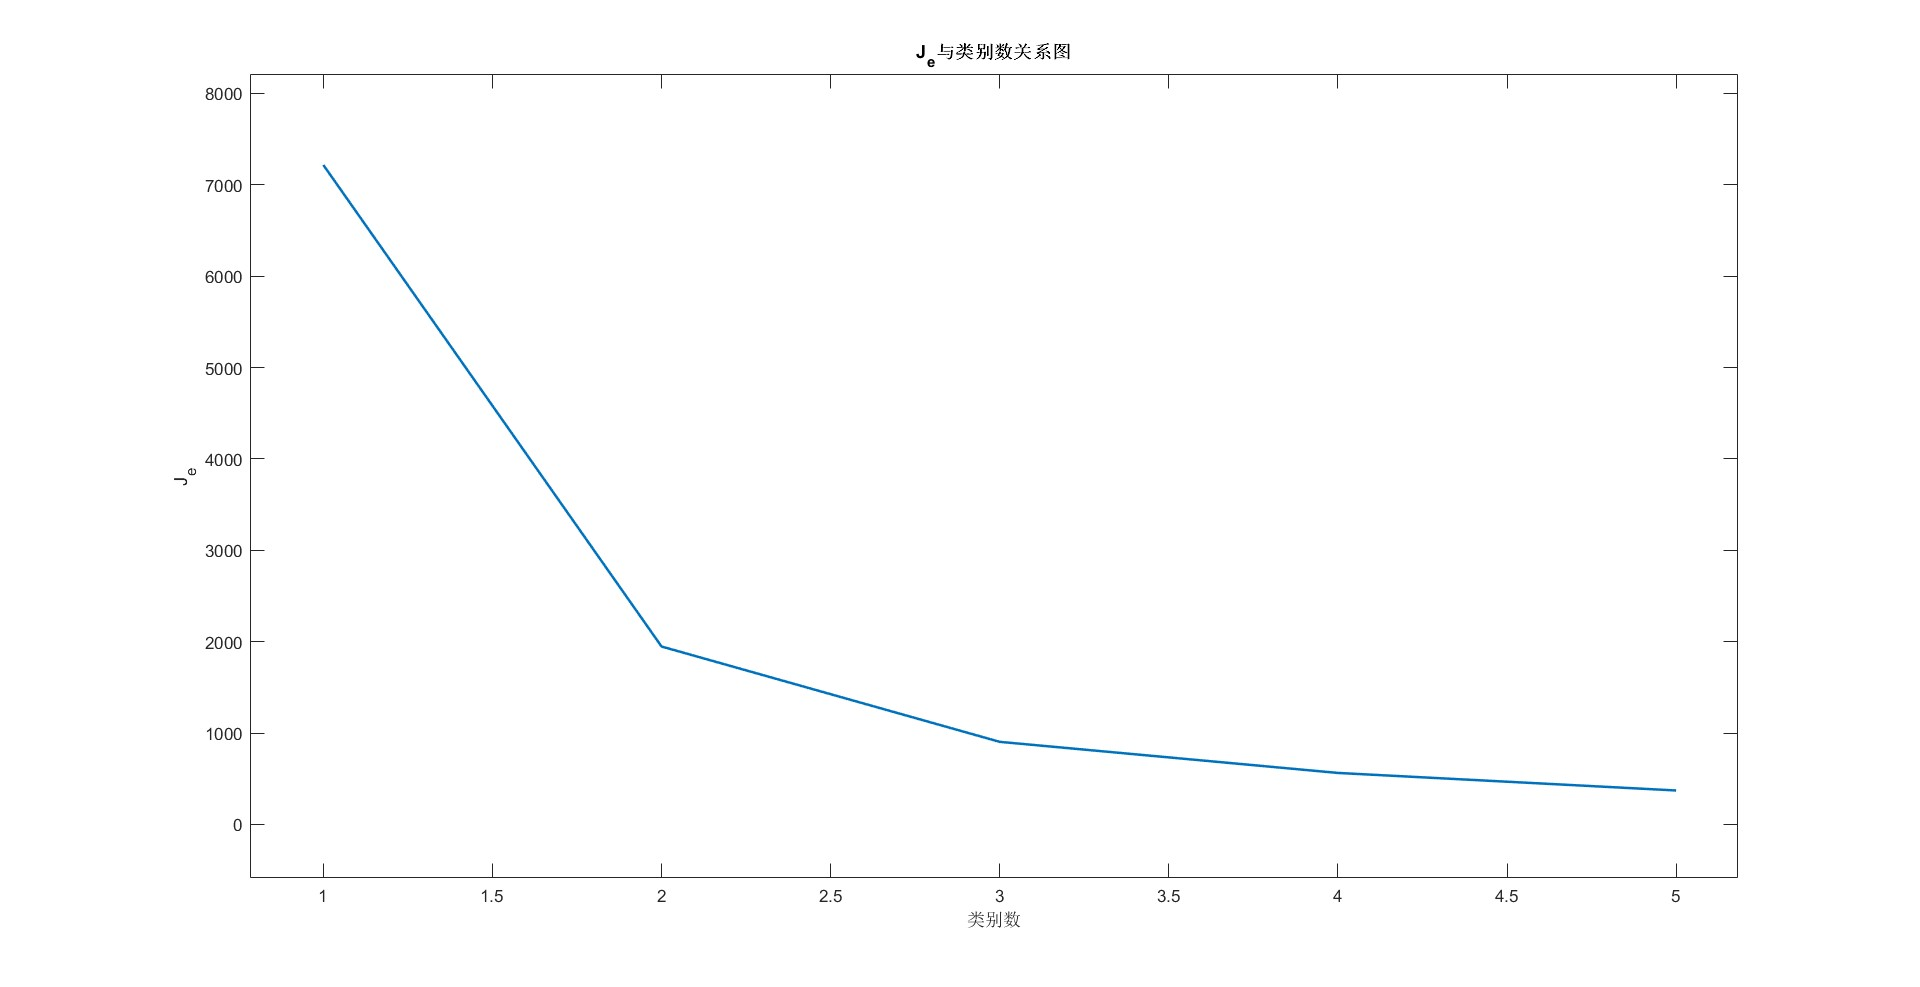
\includegraphics[width=1\textwidth]{image/Figure08.jpg}
    \caption{$J_e$随类别数的变化}
    \label{Figure08}
\end{figure}

\subsection{要求3}
层次聚类法所得系统树图如下。(为什么聚类结果很差?)

\begin{figure}[H]
    \centering
    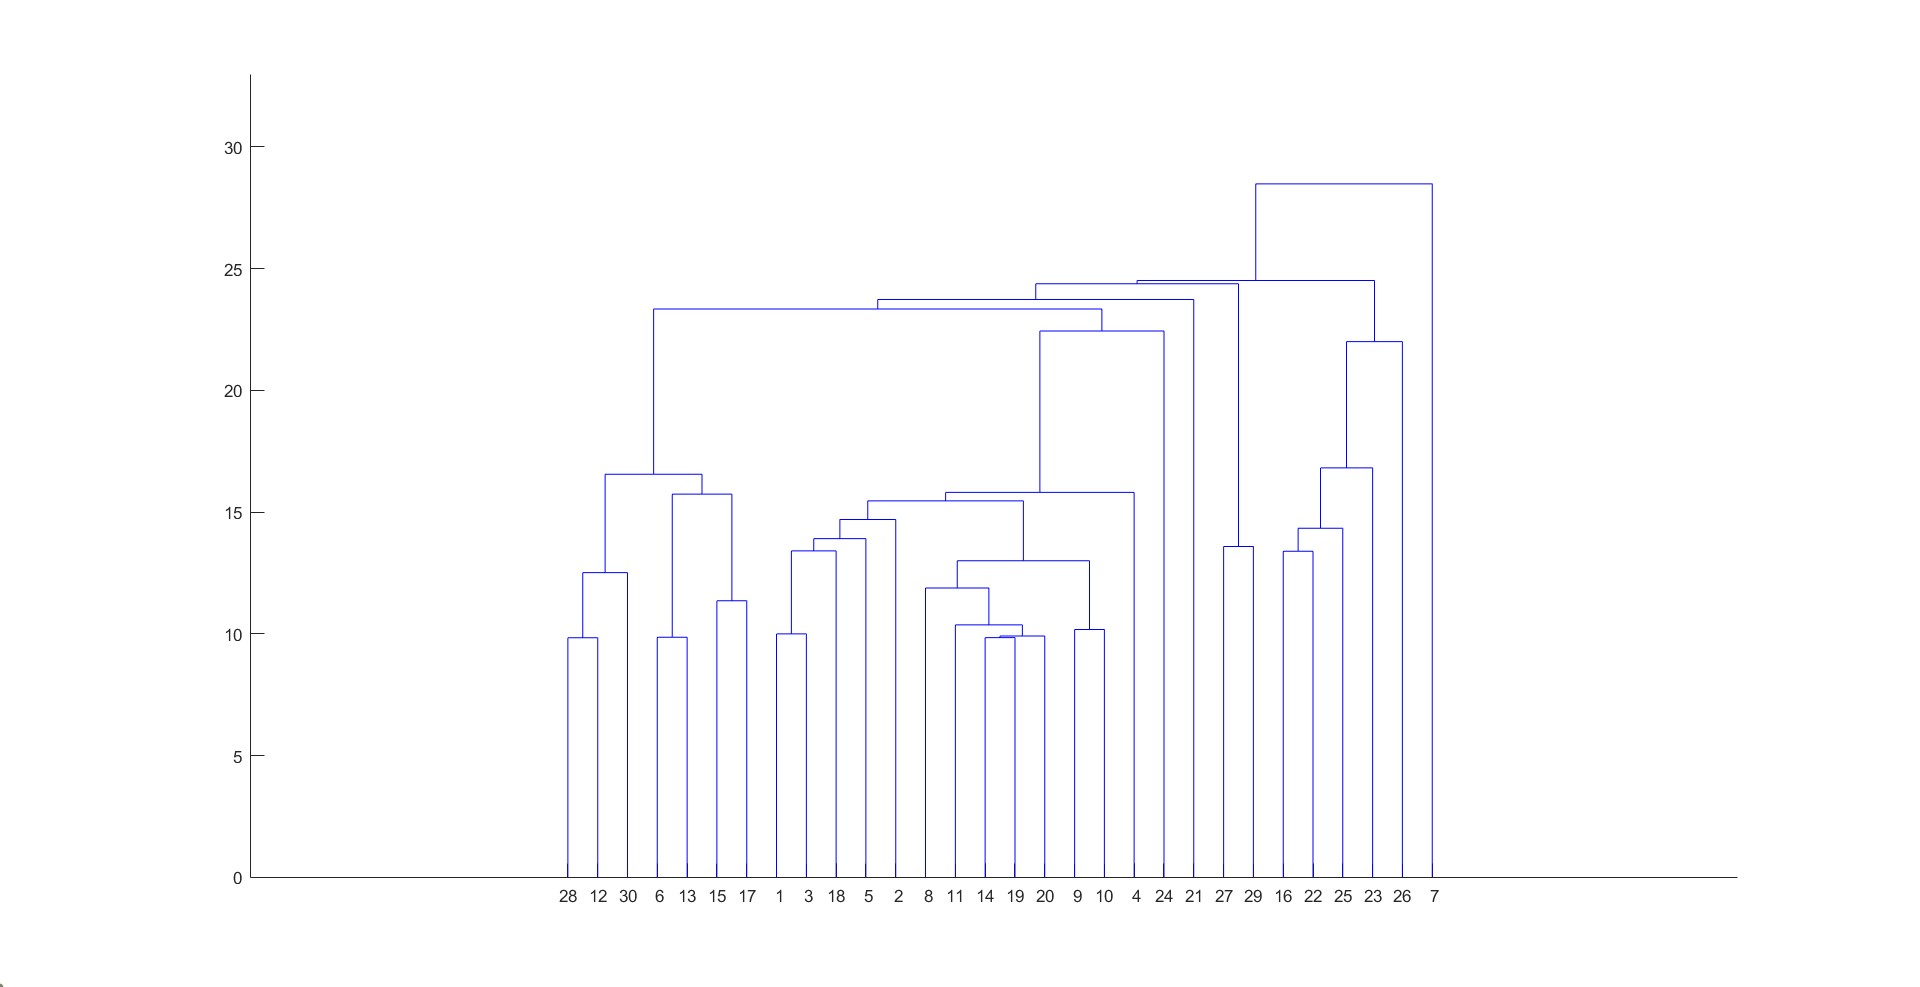
\includegraphics[width=1\textwidth]{image/Figure09.jpg}
    \caption{层次聚类聚类树}
    \label{Figure09}
\end{figure}

\subsection{要求4}
首先选择m=1.5,c=2进行聚类,得到结果如下:

\begin{figure}[H]
    \centering
    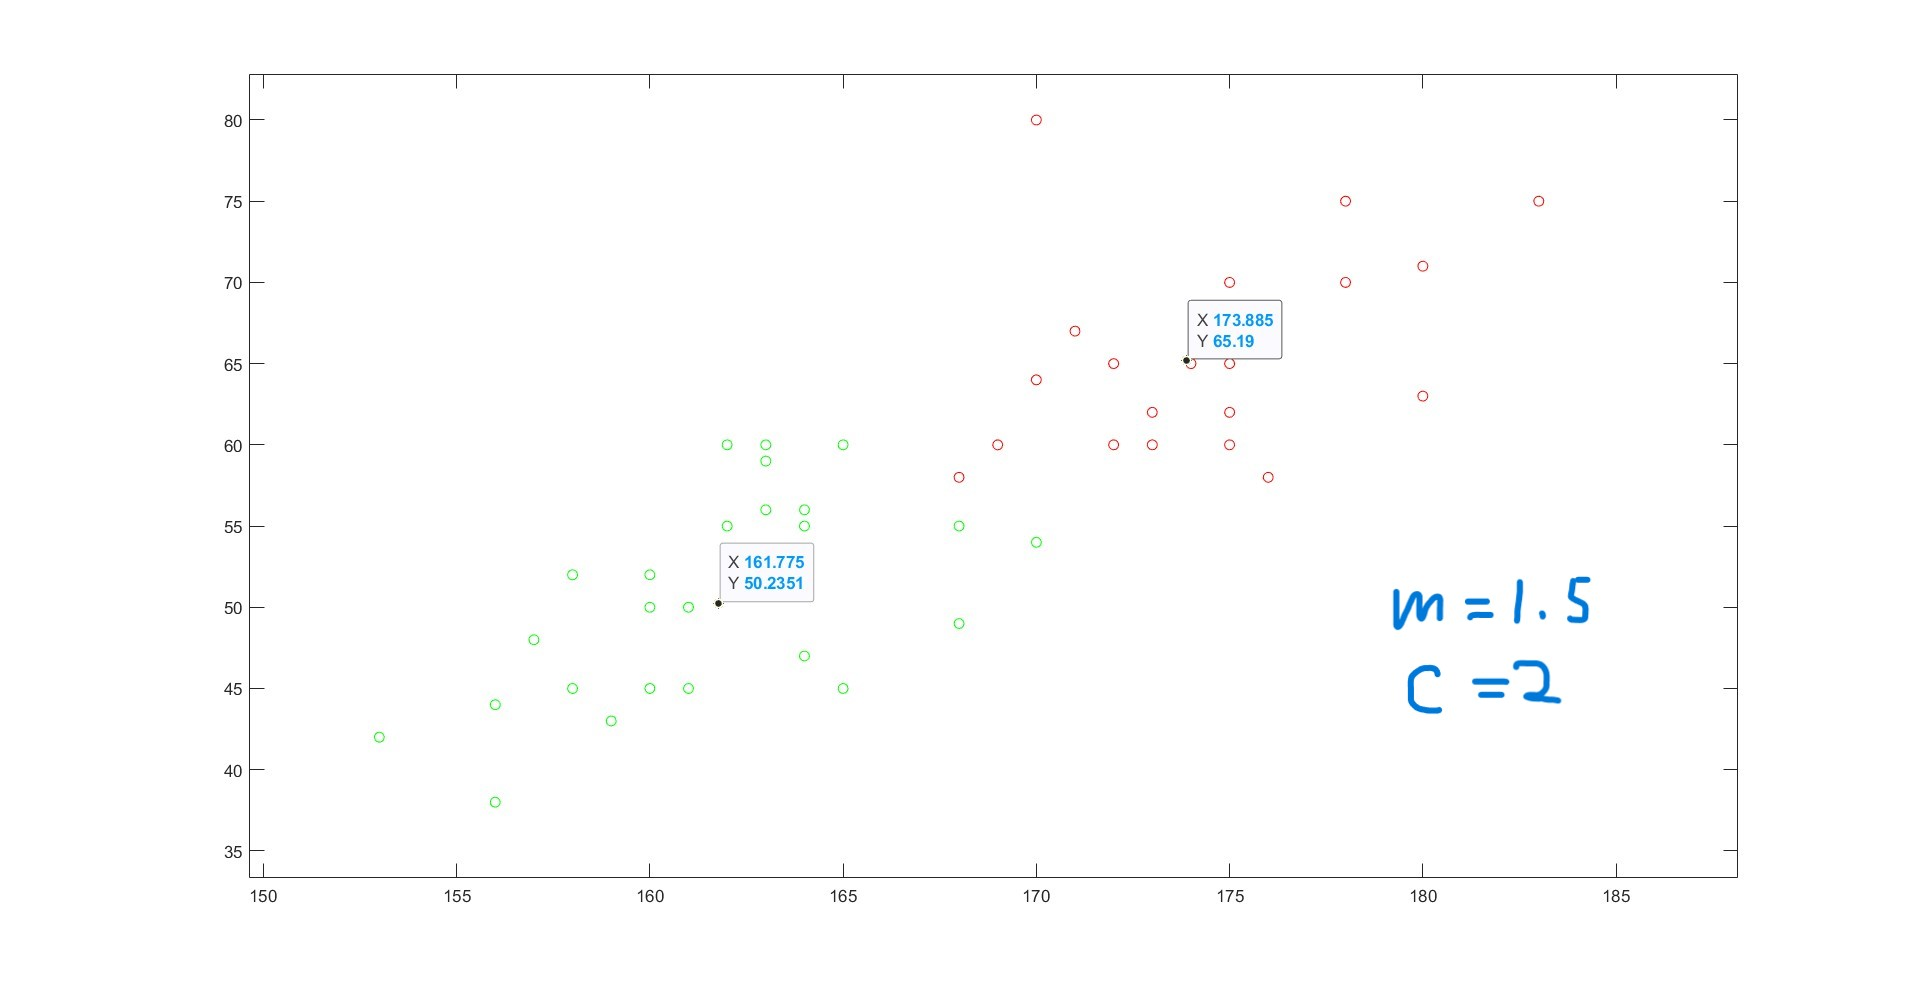
\includegraphics[width=1\textwidth]{image/Figure10_1.jpg}
    \caption{m=1.5,c=2聚类结果}
    \label{Figure10_1}
\end{figure}
\begin{figure}[H]
    \centering
    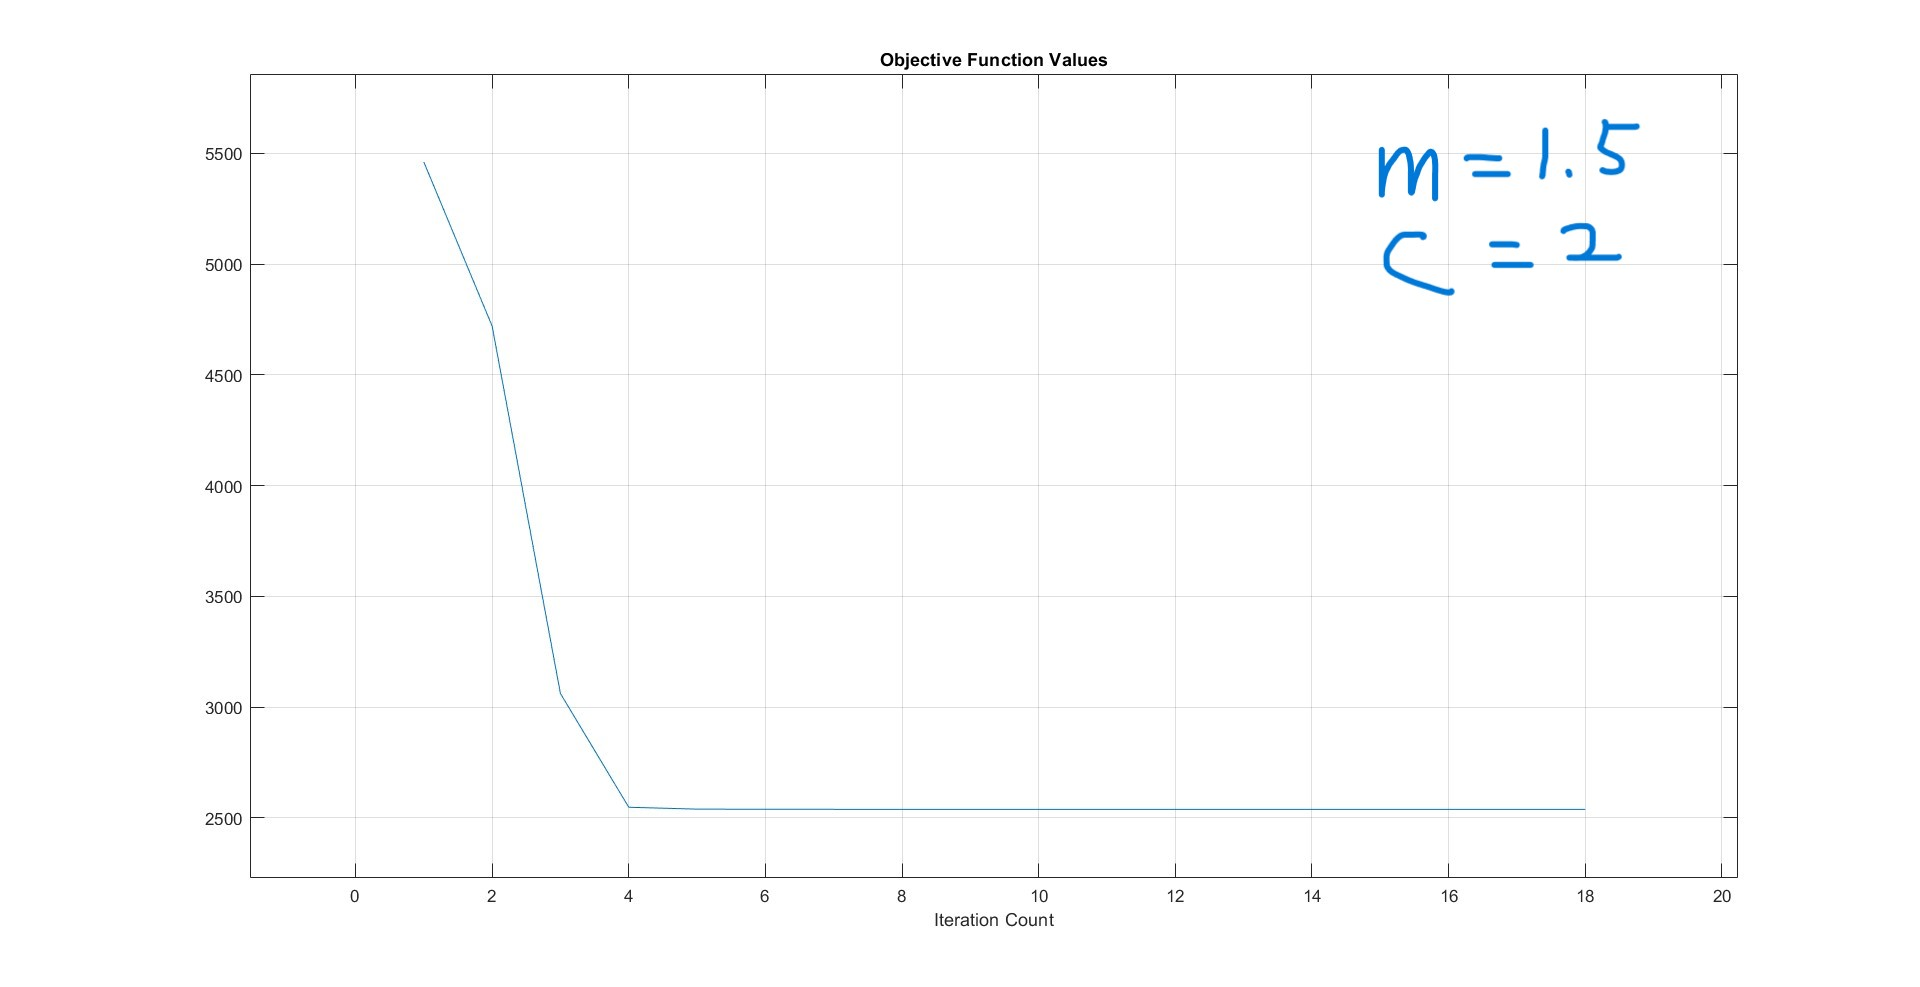
\includegraphics[width=1\textwidth]{image/Figure10_2.jpg}
    \caption{m=1.5,c=2目标函数obj\_fcn变化}
    \label{Figure10_2}
\end{figure}

选择m=2,c=2进行聚类,得到结果如下:

\begin{figure}[H]
    \centering
    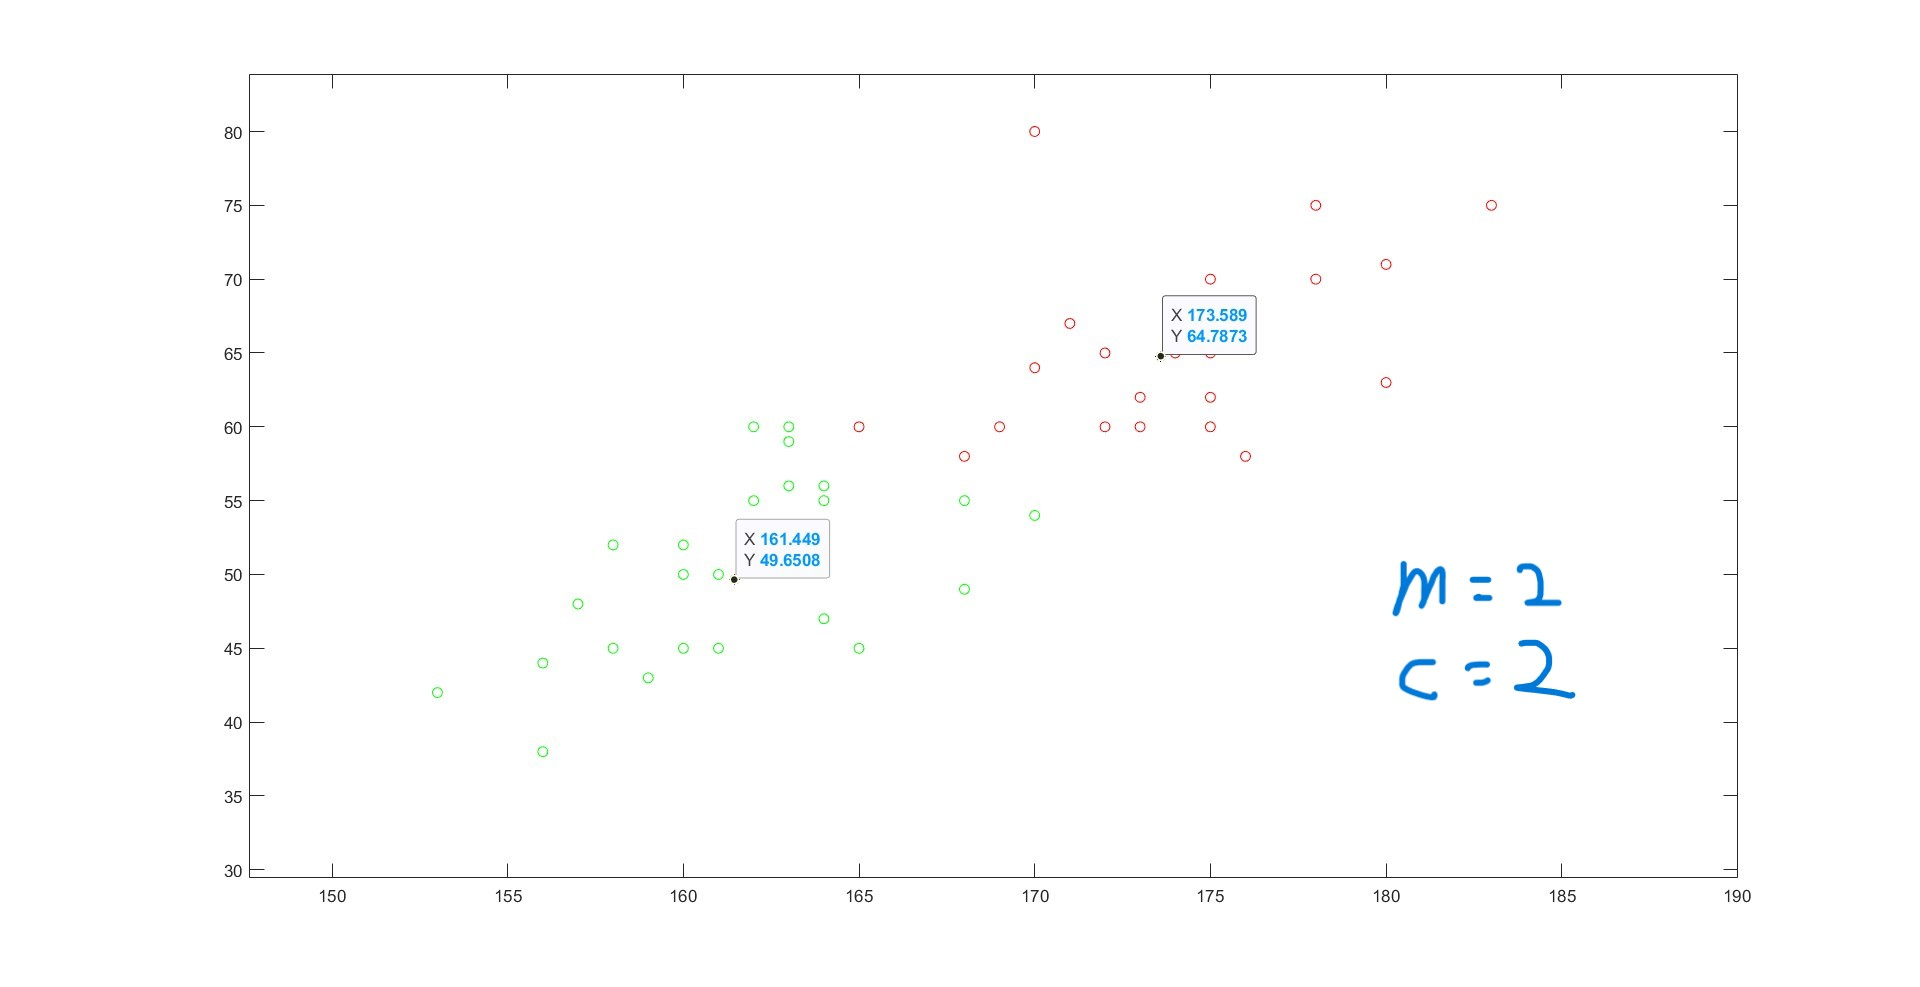
\includegraphics[width=1\textwidth]{image/Figure11_1.jpg}
    \caption{m=2,c=2聚类结果}
    \label{Figure11_1}
\end{figure}
\begin{figure}[H]
    \centering
    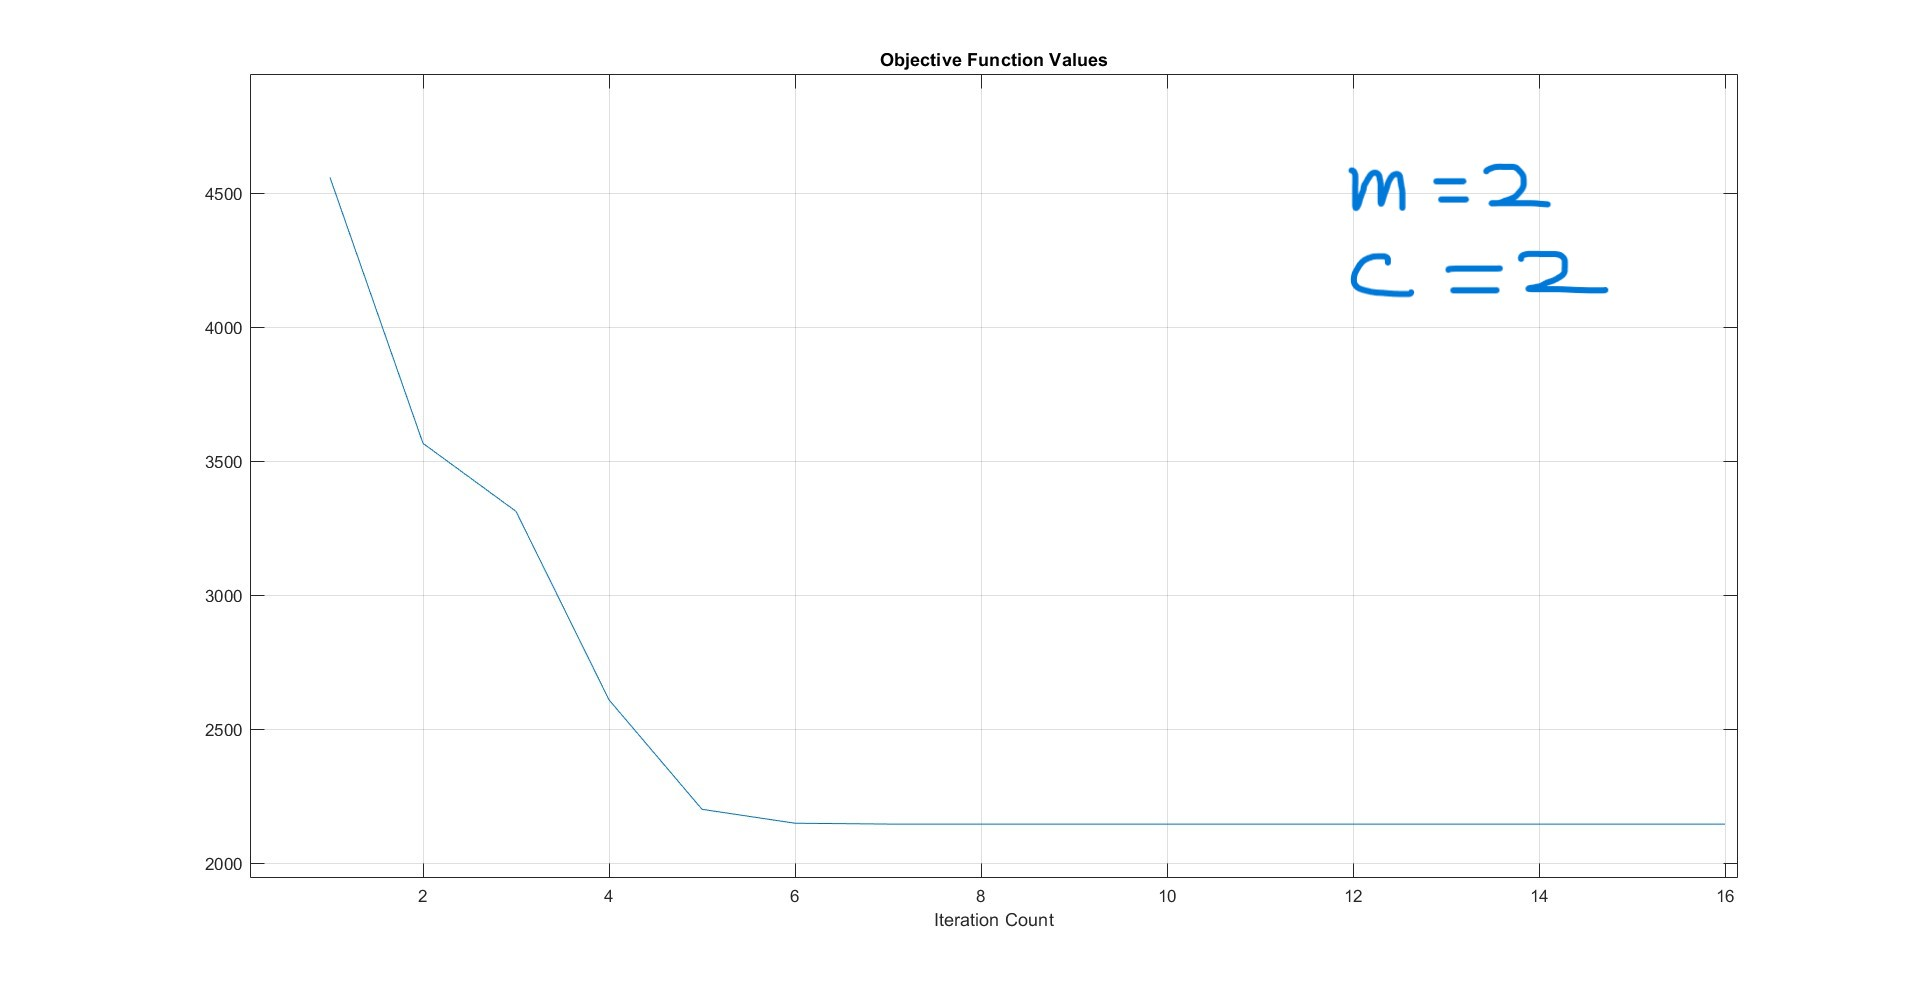
\includegraphics[width=1\textwidth]{image/Figure11_2.jpg}
    \caption{m=2,c=2目标函数obj\_fcn变化}
    \label{Figure11_2}
\end{figure}


选择m=3,c=2进行聚类,得到结果如下:

\begin{figure}[H]
    \centering
    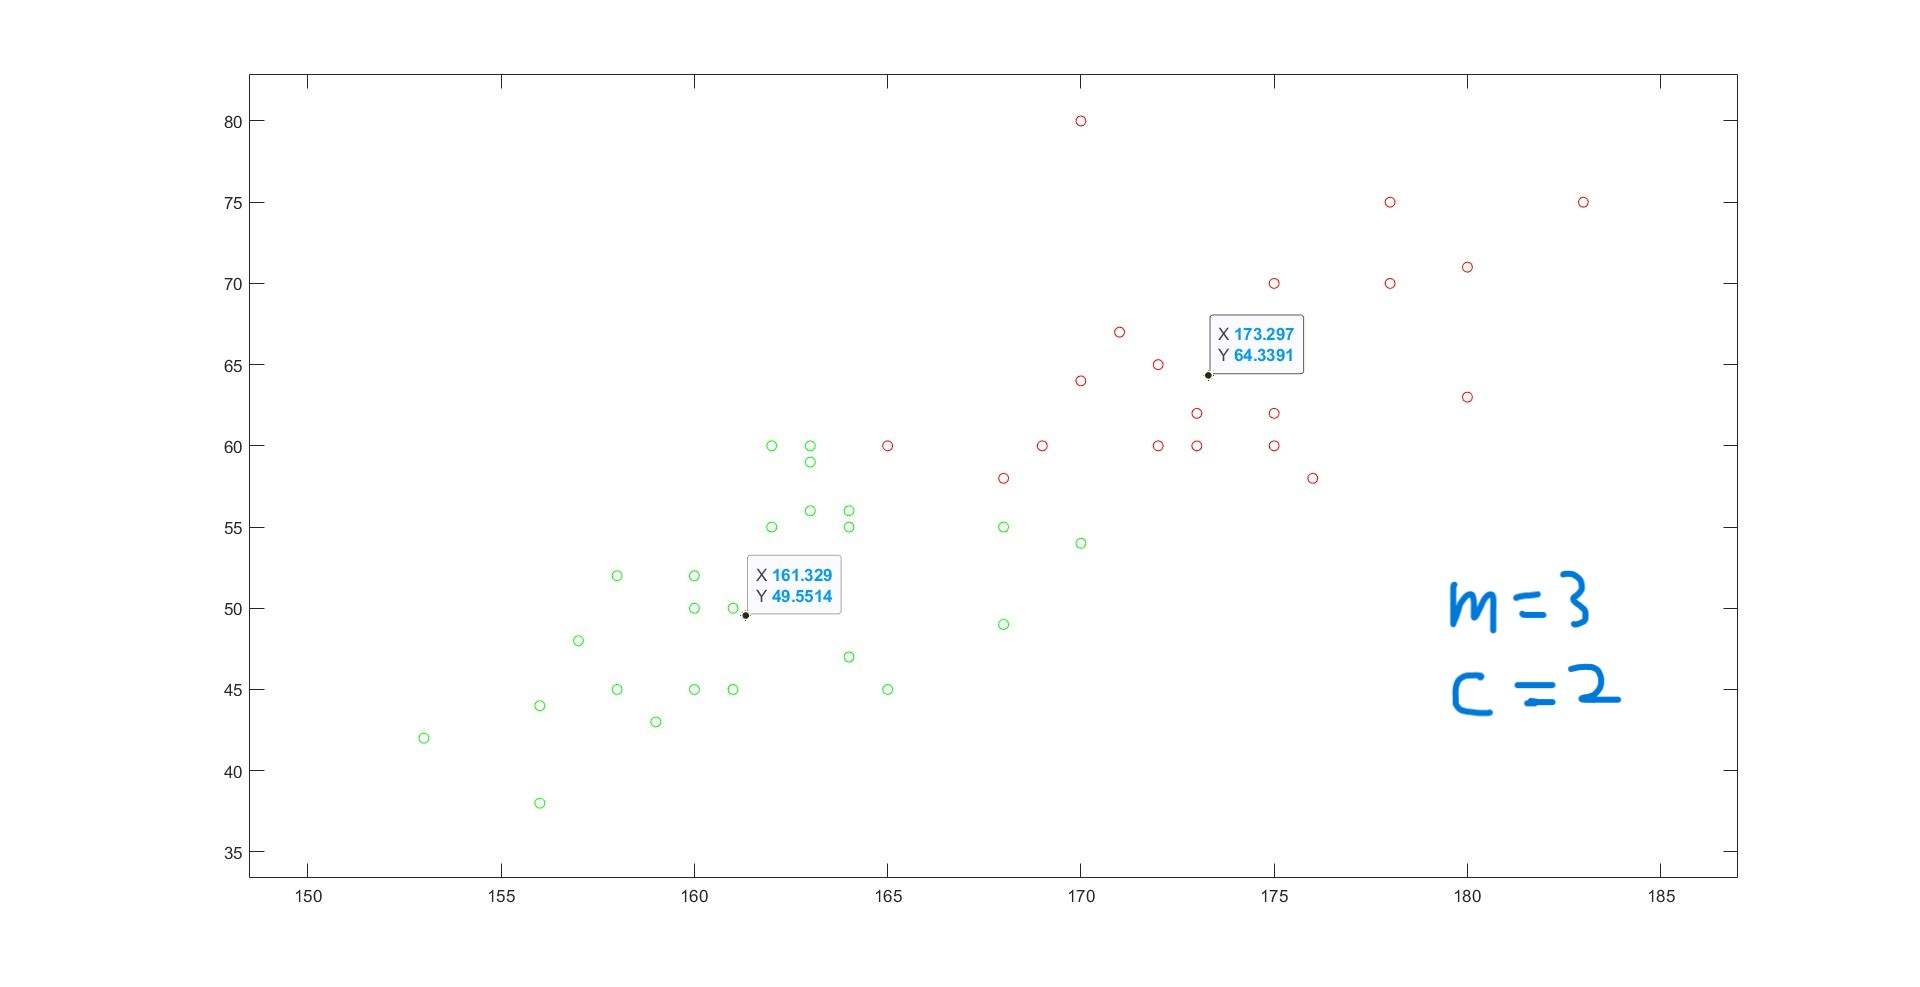
\includegraphics[width=1\textwidth]{image/Figure12_1.jpg}
    \caption{m=3,c=2聚类结果}
    \label{Figure12_1}
\end{figure}
\begin{figure}[H]
    \centering
    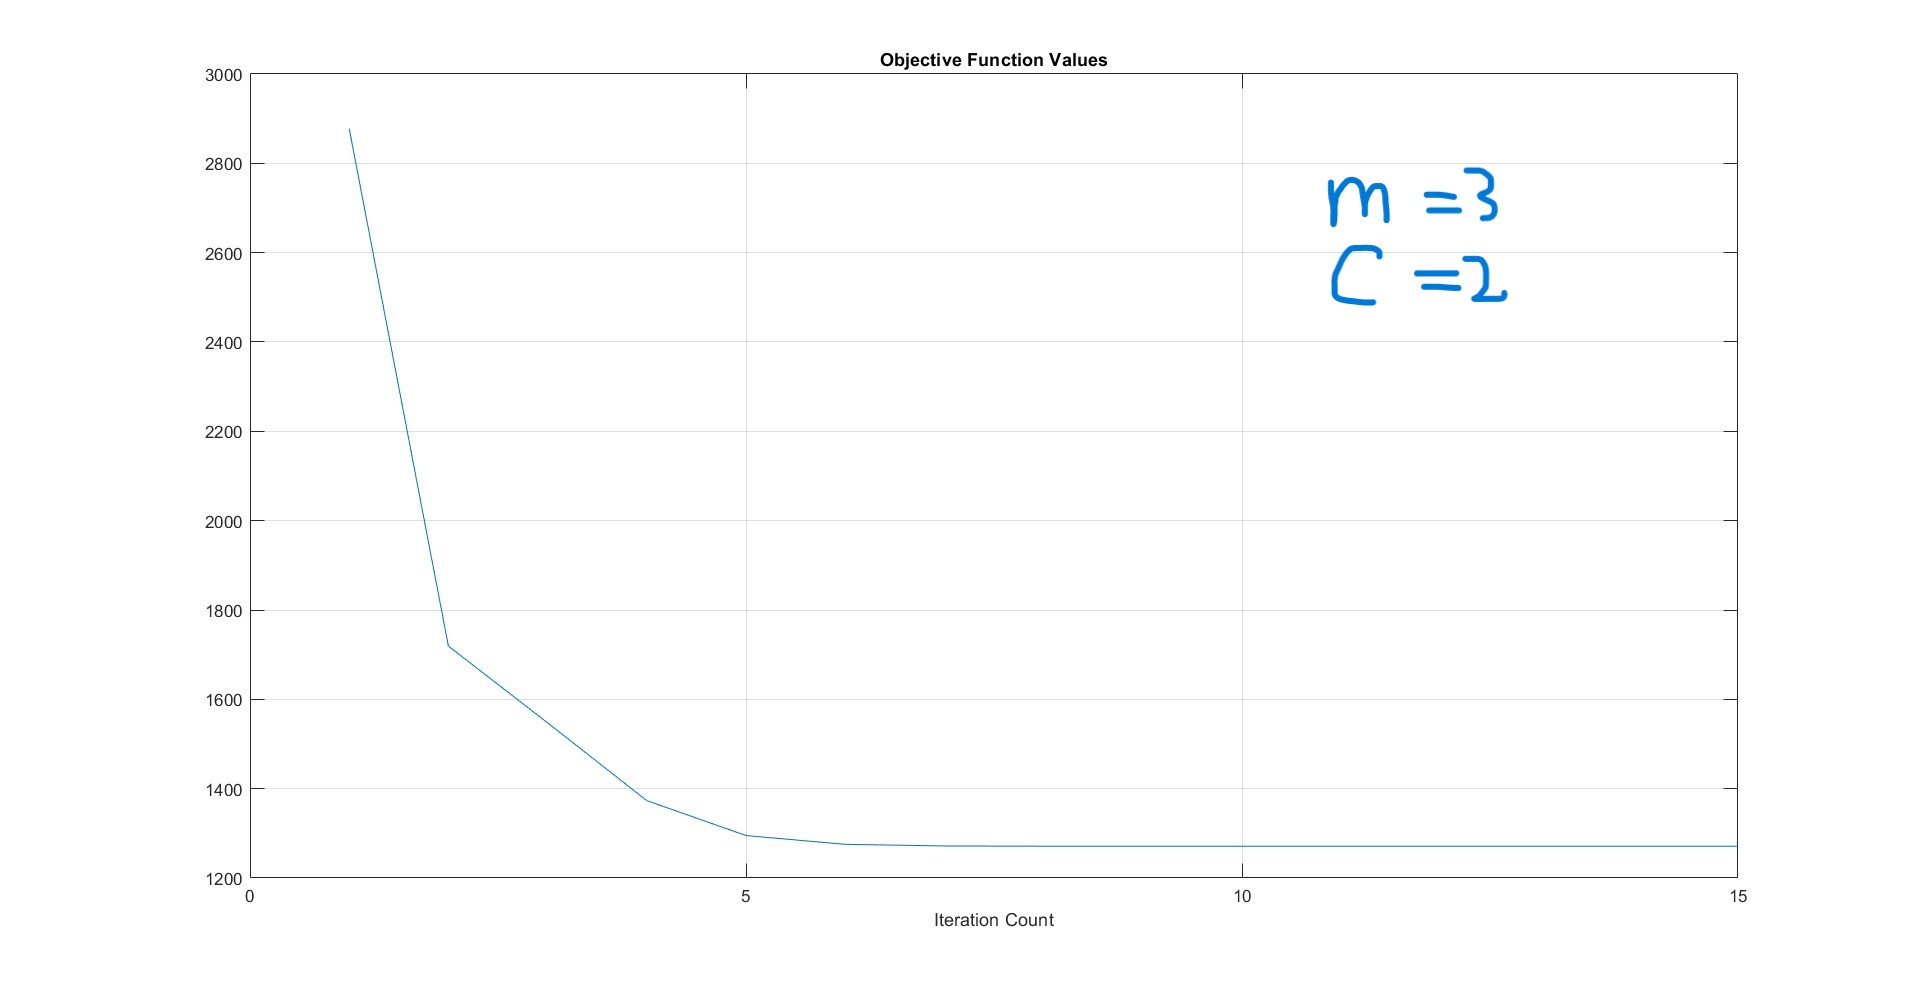
\includegraphics[width=1\textwidth]{image/Figure12_2.jpg}
    \caption{m=3,c=2目标函数obj\_fcn变化}
    \label{Figure12_2}
\end{figure}


选择m=1.5,c=3进行聚类,得到结果如下:

\begin{figure}[H]
    \centering
    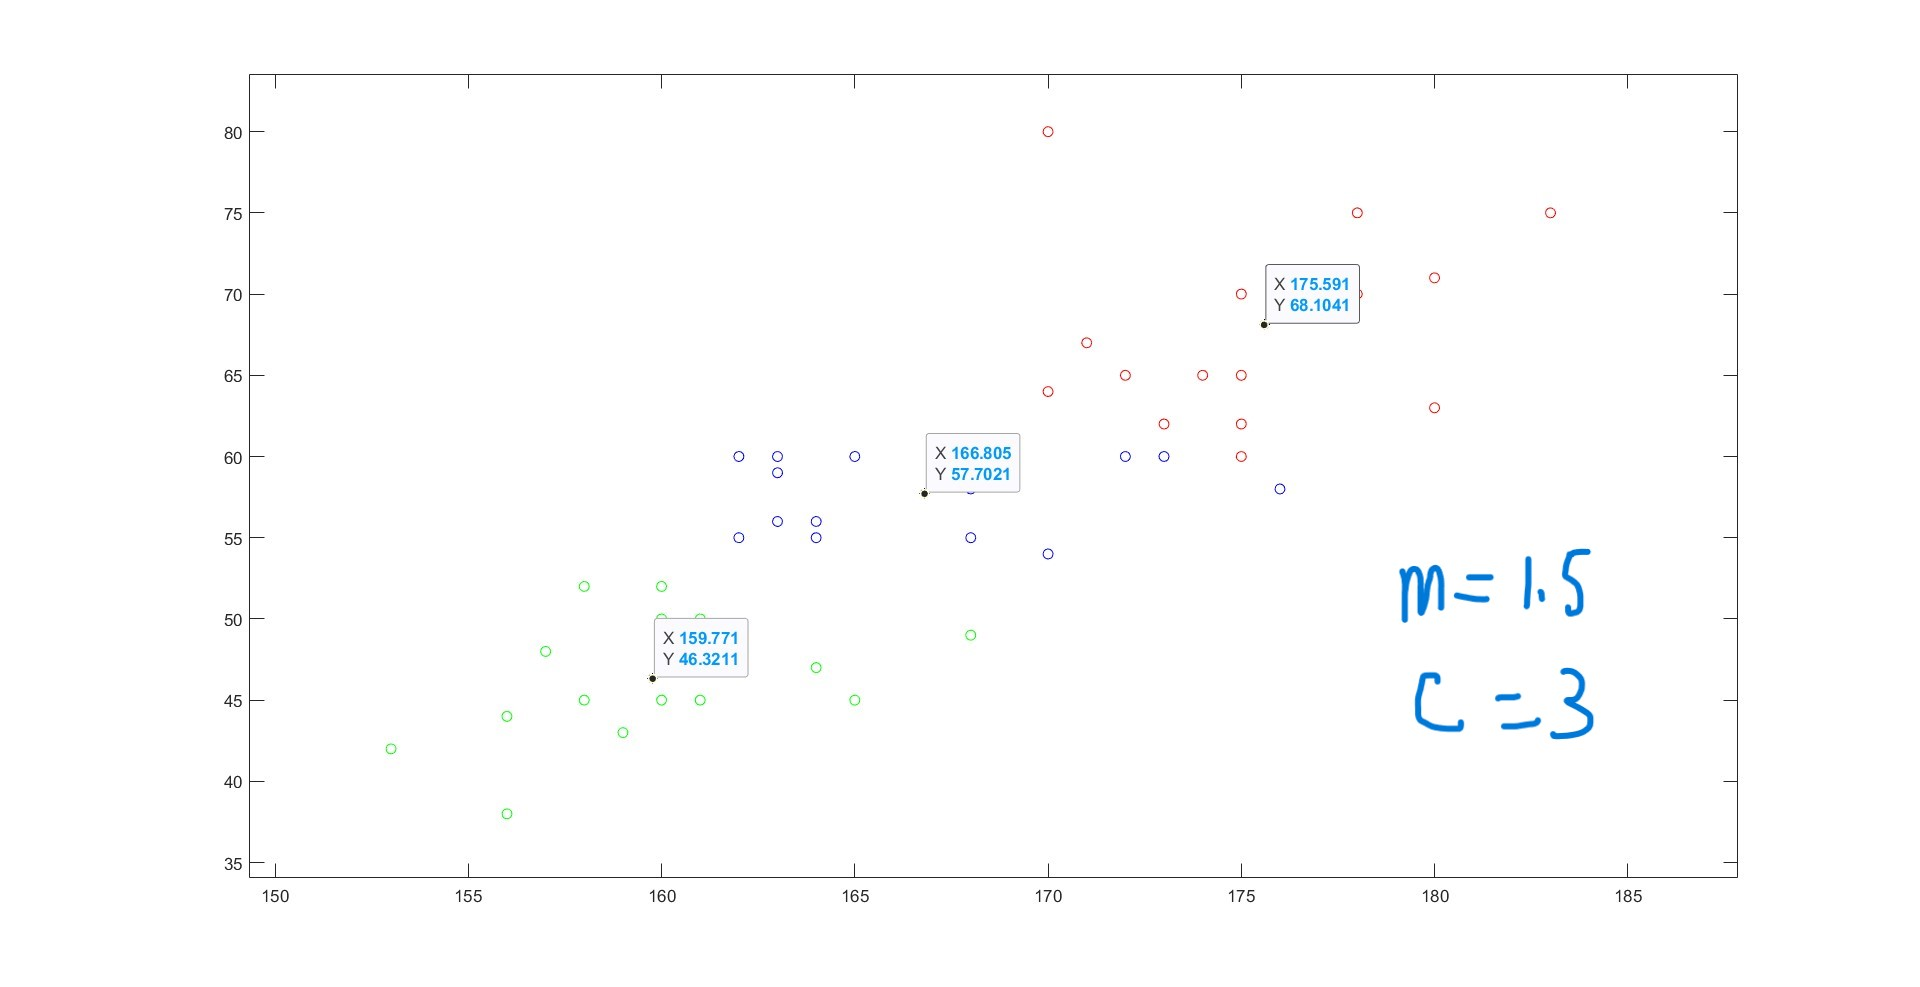
\includegraphics[width=1\textwidth]{image/Figure13_1.jpg}
    \caption{m=1.5,c=3聚类结果}
    \label{Figure13_1}
\end{figure}
\begin{figure}[H]
    \centering
    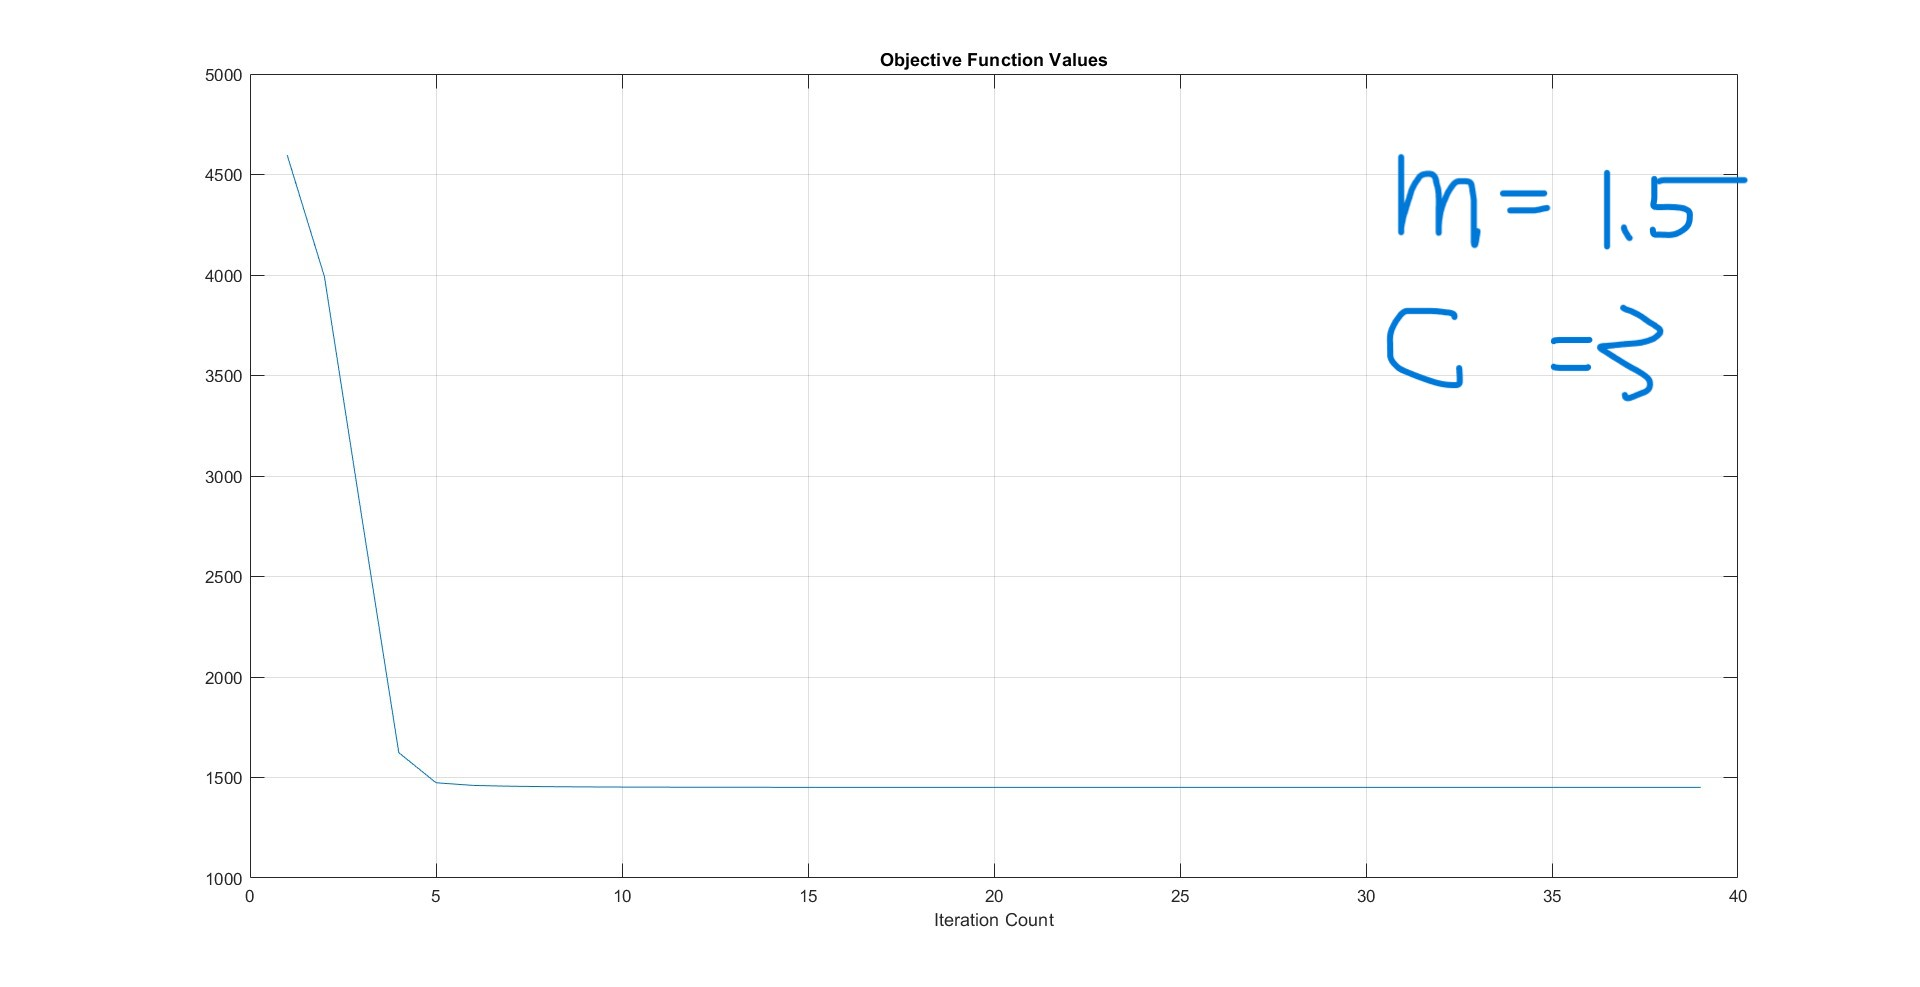
\includegraphics[width=1\textwidth]{image/Figure13_2.jpg}
    \caption{m=1.5,c=3目标函数obj\_fcn变化}
    \label{Figure13_2}
\end{figure}


当m分别取2,1.5,2.5,C为2时,可以看出分类结果大致相同,但目标函数obj\_fcn曲线在m的不同取值下有明显变化。

根据查阅的相关资料,在实际大多数应用中,m最佳取值范围是$(1.5,2.5)$

\subsection{要求5}
通过观察遗传学数据注意到,父母与子女的身高体重是一种拟合较好的线形关系,但仍然存在例外现象:矮个的人的儿子比其父要高,身材较高的父母所生子女的身高将回降到人的平均身高。当父母身高走向极端(或者非常高,或者非常矮)的人的子女,子女的身高不会象父母身高那样极端化,其身高要比父母们的身高更接近平均身高。高尔顿选用“回归”一词,把这一现象叫做“向平均数方向的回归”。但也存在外界环境对子女身高体重的影响,这部分对于普遍数据偏差不大。所以对聚类分析来说,父母的数据对分类结果的趋势影响不大。
\section{心得体会}
通过本次上机实验,我加深了对C-means聚类算法、层次聚类法和FCM聚类法的理解。并编程实现了三种算法。同时,对MATLAB编程更加熟悉。

在本次上机过程中,遇到了很多问题,通过查询资料和与同学讨论,逐一解决或避开问题,提高了解决问题的能力。同时更加深刻的认识到,官方文档才是解决问题的‘真理’,CSDN与百度内容质量参差不齐,很容易在其上浪费大量时间。但是官方文档大部分为英文,很少有翻译为中文的文档,所以,学好英语才能更好地学习技术。
\newpage

\section*{附录}
\subsection*{C-means}
\lstset{language=Matlab}
\lstset{breaklines}%自动将长的代码行换行排版
\begin{lstlisting}
clear
clc
%载入数据,绘图。
load('x.mat');
load('male.mat');
load('female.mat');
figure;
plot(male(:,1),male(:,2),'color','b','LineStyle','none','Marker','o');
hold on;
plot(female(:,1),female(:,2),'color','r','LineStyle','none','Marker','o');
hold on;
xlabel('身高/cm');
ylabel('体重/kg');
k = 1;%类别数选择

%初始质心坐标选择
%C=1
matric=[170,54];

%C = 2;
%matric=[163,60;153,42];%01
%matric=[183,75;170,54];%02
%matric=[183,75;153,42];%03

%C = 3;
%matric=[183,75;170,54;153,42];

%C = 4;
%matric=[183,75;170,54;163,60;153,42];

%C = 5;
%matric=[183,75;170,54;163,60;153,42;172,60];

%真正的代码就这一句,如果不能用封装函数,需要重写。
[idx,cen,sumD,D] = kmeans(x,k,'Start',matric);

%silhouette(x,idx); %轮廓值/轮廓系数---衡量聚类分析好坏的一个指标

%把图像画出来
color=['r','g','b','c','m','y'];


figure,
for i=1:k
    plot(x(idx==i,1),x(idx==i,2),'color',color(i),'LineStyle','none','Marker','o')
    hold on
end
xlabel('身高/cm');
ylabel('体重/kg');
title('C-means'); 

% %计算J_e 1
% J_e = 0;
% for j=1:k
%     J_tmp = [x(idx == i,1)-cen(i,1) x(idx == i,2)-cen(i,2)];
%     J_e = J_e + sum(sum(J_tmp.^2));
% end

%计算J_e 2
J_e = norm(sumD);


%显示质心坐标
plot(cen(:,1),cen(:,2),'Color','k','LineStyle','none','Marker','*')
hold off
grid on


%%绘制J_e与类别数关系图
Je = [7.2171e+03,1.9466e+03,903.2275,562.9040,370.8981];
c=[1,2,3,4,5];
figure;
plot(c,Je,'LineWidth',1.5);
xlabel('类别数')
ylabel('J_e')
title('J_e与类别数关系图')

\end{lstlisting}
\subsection*{层次聚类}
\lstset{language=Matlab}
\lstset{breaklines}%自动将长的代码行换行排版
\begin{lstlisting}
%参考代码:
%https://ww2.mathworks.cn/help/stats/cluster.html
% 载入数据
clear;
clc;
load('x.mat');
k = 2; 
% 计算前边点与后边点距离
disVector = pdist(x);  % pdist之后的Y是一个行向量,15个元素分别代表X点之间的距离
 
% 转换成方阵
disMatrix = squareform(disVector);
 
% 确定层次聚类树 
treeCluster = linkage(disMatrix);
 
% 可视化聚类树
dendrogram(treeCluster);
 
% 聚类下标
idx = cluster(treeCluster,'maxclust',k); 
 
% 画图
color=['r','g','b','c','m','y'];
figure,
for i=1:k
    plot(x(idx==i,1),x(idx==i,2),'color',color(i),'LineStyle','none','Marker','o')
    hold on
end
title('Hierarchical'); 

\end{lstlisting}

\subsection*{FCM}
\lstset{language=Matlab}
\lstset{breaklines}%自动将长的代码行换行排版
\begin{lstlisting}
clear;
load('x.mat');
k=3;%分类类别数
m=1.5;%m值的选择
[center,U,obj_fcn] = fcm(x,k,m);

maxU = max(U); 

%画图
color=['r','g','b','c','m','y']; 
figure;
for i=1:k
    plot(x(U(i,:) == maxU,1),x(U(i,:) == maxU,2),'marker','o','LineStyle','none','color',color(i));
    hold on;
end

plot(center(:,1),center(:,2),'Color','k','LineStyle','none','Marker','*')

%随迭代次数变化
figure
plot(obj_fcn)
title('Objective Function Values')   
xlabel('Iteration Count')

hold off;
grid on;


\end{lstlisting}
\newpage
\includepdf[pages={4-13}]{HandWrite.pdf} 
\end{document}